\chapter{Implementation} \label{chap:impl}

\section{Introduction}

% Proofread: 1 minor edits

Considerable research effort has been expended over the past 60 years to produce efficient flow algorithms, as discussed in \cref{sec:intro-challenges} and \cref{sec:intro-related-work}. My approach has been to embrace prior work rather than attempting to supplant it, adapting existing algorithms to improve performance for the special case of flow scheduling.

Two strategies seemed particularly promising. \emph{Approximate} solutions to the problem can be found, described in \cref{sec:impl-approx}. Existing algorithms always seek to find optimal solutions: for flow scheduling, we may be happy to trade optimality for reduced scheduling latency. Alternatively, the problem can be solved \emph{incrementally}, outlined in \cref{sec:impl-incremental}. The network remains largely unchanged between runs of the scheduler. Significant performance improvements can be realised by reoptimising from the last optimal solution found. 

These strategies are not solution methods in themselves. Rather, they suggest modifications that can be made to existing minimum-cost flow algorithms. \Cref{table:impl-application-summary} lists the algorithms I implemented, alongside the strategy they are used in.

I analysed the complexity of each algorithm, both in the general case and for scheduling flow networks. My results are summarised in \cref{table:impl-complexity-summary}, and show that the algorithmic complexity often improves on scheduling flow networks, sometimes quite significantly: for example, successive shortest path goes from being weakly to strongly polynomial.

This chapter starts by outlining the standard each of the standard algorithms listed in \cref{table:impl-application-summary}, before going on to discuss the approximate and incremental strategy. I include proofs of correctness, and the complexity results given in \cref{table:impl-complexity-summary}. However, in the interests of brevity, these results are mostly summarised in this chapter with the proofs given in \cref{appendix:impl}. I have included proofs in the main text when they are critical to understanding the implementation of the algorithm, or where they are substantially my own work.

% eliminate section prefix
\crefformats{chapter,section,subsection,appendix,subappendix,subsubappendix}{#2#1#3}
\crefnames{chapter,section,subsection,appendix,subappendix,subsubappendix}{}{}
\begin{table}
    \centering
    \begin{tabular}{lccc}
        \textbf{Name} & \textbf{Section} & \textbf{Approximation?} & \textbf{Incremental?} \tabularnewline
        \hline
        Cycle cancelling & \Cref{appendix:impl-cc} & \xmark & \xmark \tabularnewline
        Successive shortest path & \cref{sec:impl-ssp} & \xmark & \cmark \tabularnewline
        Relaxation & \cref{sec:impl-relax} & \xmark & \cmark \tabularnewline
        Cost scaling & \cref{sec:impl-cost-scaling} & \cmark & \xmark \tabularnewline
        \hline
    \end{tabular}
    \caption[Application of flow algorithms]{How each algorithm implemented in this project was used.}
    \label{table:impl-application-summary}
\end{table}

\begin{table}
    \centering
    \begin{tabular}{lcll}
        \parbox{0.1\textwidth}{\textbf{Name} \\} & \parbox{0.1\textwidth}{\textbf{Section}\\} & \parbox{0.2\textwidth}{\centering\textbf{Complexity \\ (general)}} & \parbox{0.25\textwidth}{\centering\textbf{Complexity \\ (flow scheduling)}} \tabularnewline
        \hline
        Cycle cancelling & \Cref{appendix:impl-cc} & \hspace{1em}$O\left(nm^2CU\right)$ & \hspace{2em}$O\left(n^3CU\right)$ \tabularnewline
        Successive shortest path & \cref{sec:impl-ssp} & \hspace{1em}$O\left(nmU \lg n\right)$ & \hspace{2em}$O\left(n^2\lg n\right)$ \tabularnewline
        Relaxation & \cref{sec:impl-relax} & \hspace{1em}$O\left(nm^2CU^2\right)$ & \hspace{2em}$O\left(n^3CU\right)$ \tabularnewline
        Cost scaling - FIFO & \cref{sec:impl-cost-scaling} & \hspace{1em}$O\left(n^2m\lg(nC)\right)$ & \hspace{2em}$O\left(n^3\lg(nC)\right)$ \tabularnewline
        Cost scaling - WAVE & \cref{sec:impl-cost-scaling} & \hspace{1em}$O\left(n^3\lg(nC)\right)$ & \hspace{2em}$O\left(n^3\lg(nC)\right)$ \tabularnewline
        \hline
    \end{tabular}
    \caption[Asymptotic complexity of flow algorithms]{Summary of asymptotic complexity of flow algorithms.}
    \label{table:impl-complexity-summary}
\end{table}
\crefsections

\section{Cycle cancelling algorithm} \label{sec:impl-cycle-cancelling}

% Proofread: 1 minor edits

My implementation began with cycle cancelling, a simple flow algorithm due to Klein~\cite{Klein:1967}. Its performance is exponential in the worst case, and so is not a viable option for a high-performance flow solver. However, its simplicity allowed me to implement it early on in the project. This prototype enabled me to verify that I had correctly designed and implemented other classes, such as graph data structures and a parser. Since it is not used in the final version of Hapi, I describe the algorithm in \cref{appendix:impl-cc}.
\footnotetext{Strongly polynomial variants exist~\cite{Goldberg:1989,Sokkalingam:2000}, but are still slow.}  

\section{Successive shortest path algorithm} \label{sec:impl-ssp}

% Proofread: 1 major edits, 2 minor edits

In general, this algorithm runs in weakly polynomial time. However, for the class of networks produced by flow schedulers this improves to a strongly polynomial time bound of $O(n^2 \lg n)$. Successive shortest path lends itself readily to an incremental implementation (see \cref{sec:impl-incremental}), but is inappropriate for an approximate solver.

%PROOFREAD: XXX -- inserted page break here for SSP->Algo Description
\newpage

\subsection{Algorithm description}

\begin{figure}
    \begin{subfigure}[c]{0.5\textwidth}
        \centering
        %%%%%%%%%%%%%%%%%%%%%%%%%%%%%%%%%%%%%%%%%%%
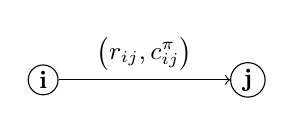
\begin{tikzpicture}[nodes={font=\bf\small}, scale=0.65]
%  \draw [help lines] (-1,-1) grid (8,5);o

\tikzstyle{tasknode}=[%
  draw,
  circle,
  minimum width=0.4,
  inner sep=0.5mm,
]

% nodes
\node [tasknode] (i) at (0, 0) {i};
\node [tasknode] (j) at (4, 0) {j};

\path [draw, ->] (i) -- node[above] {$\left(r_{ij},c_{ij}^{\pi}\right)$} (j);

\end{tikzpicture} 
%%%%%%%%%%%%%%%%%%%%%%%%%%%%%%%%%%%%%%%%%%%

        \caption{Notation: each arc is labelled with residual capacity and reduced cost.} 
    \end{subfigure}
    \begin{subfigure}[c]{0.5\textwidth}
        %%%%%%%%%%%%%%%%%%%%%%%%%%%%%%%%%%%%%%%%%%%
\begin{tikzpicture}[nodes={font=\bf\small}, scale=0.65]
%  \draw [help lines] (-1,-1) grid (8,5);o

\tikzstyle{tasknode}=[%
  draw,
  circle,
  minimum width=0.4,
  inner sep=0.5mm,
]

% T_0,0
\node [tasknode, black!70!green] (t00) at (0,6.5) {T$_0^0$};
% T_0,1
\node [tasknode, black!70!green] (t01) at (0,4.5) {T$_1^0$};

% X
\node [draw, rectangle, brown] (x) at (5.0,3.5) {X};

% M_0 & M_1
\node [draw, rectangle, blue] (m0) at (10.0,6.5) {M$_0$};
\node [draw, rectangle, blue] (m1) at (10.0,4.5) {M$_1$};
\node [draw, rectangle, blue] (m2) at (10.0,2.5) {M$_2$};

% sink
\node [draw, regular polygon, regular polygon sides=6] (s) at (12, 3.5) {S};

% U_0
\node [draw, rectangle, red] (u0) at (5.0,7.0) {U$^0$};

% Tasks to X
\path [draw, ->] (t00) -- node[below, sloped] {1} (x);
\path [draw, ->] (t01) -- node[below, sloped] {1} (x);

% Tasks to U_i
\path [draw, ->] (t00) -- node[above, sloped] {5} (u0);
\path [draw, ->] (t01) -- node[above, sloped] {5} (u0);

% X to machines
\path [draw, ->] (x) -- node[below, sloped] {} (m0);
\path [draw, ->] (x) -- node[below, sloped] {} (m1);
\path [draw, ->] (x) -- node[below, sloped] {} (m2);

% Machines to sink
\path [draw, ->, red] (m0) -- node[above, sloped] {} (s);
\path [draw, ->, red] (m1) -- node[below, sloped] {} (s);
\path [draw, ->] (m2) -- node[below, sloped] {} (s);

% U_i to sink
\begin{scope}[decoration={post length=4pt},rounded corners=4mm]
  \path [draw, ->] (u0) -- ++(1.5,0.5) -- node[below, sloped] {} ++(6,0) -- ++(1,-0.5) -- (s);
\end{scope}

% running tasks
\path [draw, ->, dotted, red] (t00) edge[out=-30, in=180, looseness=1] node[above, sloped] {1} (m0);
\path [draw, ->, dotted, red] (t01) edge[out=15, in=180, looseness=1] node[above, sloped] {1} (m1);

\end{tikzpicture} 
%%%%%%%%%%%%%%%%%%%%%%%%%%%%%%%%%%%%%%%%%%%

        \caption{Initial network.}
    \end{subfigure}
    \begin{subfigure}[c]{0.5\textwidth}
        \input{figures/flow/ssp/first_pi}
        \caption{SSSP problem solved from \textbf{A}, and potentials updated.}
        \label{fig:ssp-trace:first-pi}
    \end{subfigure}
    \begin{subfigure}[c]{0.5\textwidth}
        %%%%%%%%%%%%%%%%%%%%%%%%%%%%%%%%%%%%%%%%%%%
\begin{tikzpicture}[nodes={font=\bf\small}, scale=0.65]
%  \draw [help lines] (-1,-1) grid (8,5);o

\tikzstyle{mynode}=[%
  draw,
  circle,
  minimum width=0.4,
  inner sep=0.5mm,
]

\tikzstyle{myarc}=[%
  draw,
  arrows={-Triangle[scale=1]},
  line width=1pt,
]

% nodes
\node [mynode] (a) at (0, 4) {A};
\node [mynode] (b) at (4, 8) {B};
\node [mynode] (c) at (4, 0) {C};
\node [mynode] (d) at (8, 4) {D};

% excesses
\node [left=0.5cm] at (0,4.3) {$e_1 = 2$}; % A
\node [above=0.6cm] at (4,8) {$e_2 = 0$}; % B
\node [below=0.2cm] at (4,0) {$e_3 = 0$}; % C
\node [right=0.5cm] at (8,4.3) {$e_4 = -2$}; % D

% s=A, t=D
% shortest paths:
% B: A->B (1)
% C: A->C (5)
% D : A->B->D (2)

% potentials
\node [left=0.5cm] at (0,3.7) {$\pi_1 = 0$}; % A
\node [above=0.15cm] at (4,8) {$\pi_2 = -1$}; % B
\node [below=0.65cm] at (4,0) {$\pi_3 = -5$}; % C
\node [right=0.5cm] at (8,3.7) {$\pi_4 = -2$}; % D

% (cap,cost)
\path [myarc] (a) -- node[above, sloped] {$(1,0)$} (b);
\path [myarc] (b) edge[bend left=20, looseness=1] node[below, sloped] {$(1,0)$} (a);
\path [myarc] (a) -- node[below, sloped] {$(3,0)$} (c);
\path [myarc] (b) -- node[right] {$(5, 6)$} (c);
\path [myarc] (d) -- node[above, sloped] {$(1,0)$} (b);
\path [myarc] (c) -- node[below, sloped] {$(5,4)$} (d);

\end{tikzpicture} 
%%%%%%%%%%%%%%%%%%%%%%%%%%%%%%%%%%%%%%%%%%%

        \label{fig:ssp-trace:first-augment}                
        \caption{Flow augmented along shortest path $A \to B \to D$.}
    \end{subfigure}
    \begin{subfigure}[c]{0.5\textwidth}
        %%%%%%%%%%%%%%%%%%%%%%%%%%%%%%%%%%%%%%%%%%%
\begin{tikzpicture}[nodes={font=\bf\small}, scale=0.65]
%  \draw [help lines] (-1,-1) grid (8,5);o

\tikzstyle{mynode}=[%
  draw,
  circle,
  minimum width=0.4,
  inner sep=0.5mm,
]

\tikzstyle{myarc}=[%
  draw,
  arrows={-Triangle[scale=1]},
  line width=1pt,
]

% nodes
\node [mynode] (a) at (0, 4) {A};
\node [mynode] (b) at (4, 8) {B};
\node [mynode] (c) at (4, 0) {C};
\node [mynode] (d) at (8, 4) {D};

% excesses
\node [left=0.5cm] at (0,4.3) {$e_1 = 0$}; % A
\node [above=0.6cm] at (4,8) {$e_2 = 0$}; % B
\node [below=0.2cm] at (4,0) {$e_3 = 0$}; % C
\node [right=0.5cm] at (8,4.3) {$e_4 = 0$}; % D

% s=A, t=D
% shortest paths:
% B: A->B (0)
% C: A->C (0)
% D: A->C->B (4)

% potentials
\node [left=0.5cm] at (0,3.7) {$\pi_1 = 0$}; % A
\node [above=0.15cm] at (4,8) {$\pi_2 = -1$}; % B
\node [below=0.65cm] at (4,0) {$\pi_3 = -5$}; % C
\node [right=0.5cm] at (8,3.7) {$\pi_4 = -6$}; % D

% (cap,cost)
\path [myarc] (a) -- node[above, sloped] {$(1,0)$} (b);
\path [myarc] (b) edge[bend left=20, looseness=1] node[below, sloped] {$(1,0)$} (a);
\path [myarc] (a) -- node[below, sloped] {$(3,0)$} (c);
\path [myarc] (b) -- node[right] {$(5, 6)$} (c);
\path [myarc] (d) -- node[above, sloped] {$(1,4)$} (b);
\path [myarc] (c) -- node[below, sloped] {$(5,0)$} (d);

\end{tikzpicture} 
%%%%%%%%%%%%%%%%%%%%%%%%%%%%%%%%%%%%%%%%%%%

        \caption{SSSP problem solved from \textbf{A}, and potentials updated.}
        \label{fig:ssp-trace:second-pi}
    \end{subfigure}
    \begin{subfigure}[c]{0.5\textwidth}
        %%%%%%%%%%%%%%%%%%%%%%%%%%%%%%%%%%%%%%%%%%%
\begin{tikzpicture}[nodes={font=\bf\small}, scale=0.45]
%  \draw [help lines] (-1,-1) grid (8,5);o

\tikzstyle{mynode}=[%
  draw,
  circle,
  minimum width=0.4,
  inner sep=0.5mm,
]

\tikzstyle{myarc}=[%
  draw,
  arrows={-Triangle[scale=1]},
  line width=1pt,
]

% nodes
\node [mynode] (a) at (0, 4) {A};
\node [mynode] (b) at (4, 8) {B};
\node [mynode] (c) at (4, 0) {C};
\node [mynode] (d) at (8, 4) {D};

% excesses
\node [left=0.3cm] at (0,4.5) {\color{red} $e_A = 0$}; % A
\node [above=0.6cm] at (4,8) {$e_B = 0$}; % B
\node [below=0.2cm] at (4,0) {$e_C = 0$}; % C
\node [right=0.3cm] at (8,4.5) {\color{red} $e_D = 0$}; % D

% s=A, t=D
% shortest paths:
% B: A->B (0)
% C: A->C (0)
% D: A->C->B (4)

% potentials
\node [left=0.3cm] at (0,3.5) {$\pi_A = 0$}; % A
\node [above=0.15cm] at (4,8) {$\pi_B = -1$}; % B
\node [below=0.65cm] at (4,0) {$\pi_C = -5$}; % C
\node [right=0.3cm] at (8,3.5) {$\pi_D = -6$}; % D

% (cap,cost)
\path [myarc] (a) -- node[above, sloped] {$(1,0)$} (b);
\path [myarc] (b) edge[bend left=20, looseness=1] node[below, sloped] {$(1,0)$} (a);
\path [myarc, red] (a) -- node[below, sloped] {$(1,0)$} (c);
\path [myarc] (c) edge[bend right=20, looseness=1] node[above, sloped] {$(2,0)$} (a);
\path [myarc] (b) -- node[above right] {$(5, 6)$} (c);
\path [myarc] (d) -- node[above, sloped] {$(1,4)$} (b);
\path [myarc, red] (c) -- node[below, sloped] {$(3,0)$} (d);
\path [myarc] (d) edge[bend right=20, looseness=1] node[above, sloped] {$(2,0)$} (c);

\end{tikzpicture} 
%%%%%%%%%%%%%%%%%%%%%%%%%%%%%%%%%%%%%%%%%%%

        \label{fig:ssp-trace:second-augment}        
        \caption{Flow augmented along shortest path $A \to C \to D$.}
    \end{subfigure}
    \caption[Successive shortest path algorithm in action]{Step-by-step trace of the successive shortest path algorithm in action, depicting the residual network. Each node $i$ is labelled with its excess $e_i$ and potential $\pi_i$.}
    \label{fig:ssp-trace}
\end{figure}

% SOMEDAY: footnote after $t$ is bad
\begin{algorithm}
    \caption{Successive shortest path}
    \label{algo:successive-shortest-path}
    \begin{algorithmic}[1]
        \State $\mathbf{x} \gets \mathbf{0}$ and $\boldsymbol{\pi} \gets \mathbf{0}$
        \While{mass balance constraints not satisfied} \label{algo:successive-shortest-path:start-loop}
          \State choose excess vertex $s$ and deficit vertex $t$\footnotemark \label{algo:successive-shortest-path:select-active}
          % SOMEDAY: These statements are multi-line, shorten? Or at least reflow.
          \State solve SSSP problem from $s$ to all vertices in the residual network $G_{\mathbf{x}}$, with respect to the reduced costs $c^{\boldsymbol{\pi}}_{ij}$ \label{algo:successive-shortest-path:solve-sssp}
          \State let $\mathbf{d}$ denote the vector of shortest path distances, such that $d_i$ is the shortest path from $s$ to $i\in V$
          \Let{$\boldsymbol{\pi}$}{$\boldsymbol{\pi} - \mathbf{d}$} \label{algo:successive-shortest-path:update-potentials}
          \State let $P$ denote a shortest path from $s$ to $t$
          \Let{$\delta$}{$\min\left(e_s, -e_t, \min\left\{ r_{ij} \::\: (i,j) \in P\right\}\right)$} \label{algo:successive-shortest-path:compute-delta}
          \State augment $\delta$ units of flow along path $P$ \label{algo:successive-shortest-path:augment-flow}
        \EndWhile \label{algo:successive-shortest-path:end-loop}
    \end{algorithmic}
\end{algorithm}

\footnotetext{Note so long as the mass balance constraints are unsatisfied, there must exist both an excess vertex $s$ and deficit vertex $t$. This is because the total sum of excesses must equal the total sum of deficits for any feasible problem.}

The successive shortest path algorithm maintains a pseudoflow $\mathbf{x}$ (see \cref{sec:prep-flow-pseudo}) and potentials $\boldsymbol{\pi}$ satisfying reduced cost optimality (see \cref{thm:optimality-reduced-cost}), and attempts to attain feasibility. This is in contrast to the cycle cancelling algorithm, which maintains feasibility and strives to achieve optimality.

Each iteration of the algorithm identifies an excess vertex $s$ and excess vertex $t$. Next, the single-source shortest-path (SSSP) problem~\cite[ch.~24]{CLRS:2009} is solved from $s$. To maintain reduced cost optimality, the potentials $\boldsymbol{\pi}$ are updated. Finally, the pseudoflow $\mathbf{x}$ is augmented along a shortest path $P$ from $s$ to $t$. The algorithm terminates when no excess or deficit vertices exist.

The amount of flow $\delta$ sent over the path is limited by the minimum residual capacity of arcs along $P$. $\delta$ is further restricted so that a non-negative supply at $s$ and demand at $t$ are maintained. This guarantees the excess at supply vertices and deficit at demand vertices is monotonically decreasing, ensuring each iteration improves the feasibility of the flow.

\Cref{fig:ssp-trace} illustrates the operation of successive shortest path. Note that updating the potentials in \cref{fig:ssp-trace:first-pi,fig:ssp-trace:second-pi} makes the reduced cost of arcs in the shortest-path tree rooted at \textbf{A} zero, allowing the flow to be augmented in \cref{fig:ssp-trace:first-augment,fig:ssp-trace:second-augment} without violating reduced cost optimality.

\subsection{Optimisations} \label{sec:impl-ssp-optimisations}

\subsubsection{Choice of shortest-path algorithm}
The fastest known single-source shortest-path algorithms are all variants of Djikstra's algorithm~\cite[ch.~4]{Ahuja:1993}, differing in the underlying heap data structure used. The asymptotically fastest are based on Fibonacci heaps, with a complexity of $O(m + n\lg n)$. By contrast, Djikstra's algorithm has a complexity of $O(m\lg n)$ when using the popular binary heap data structure\footnotemark.
\footnotetext{Although binary and Fibonacci heaps have the same asymptotic complexity on flow scheduling networks, since $m = O(n)$ by \cref{lemma:network-num-arcs}.} 

However, computational benchmarks have found Fibonacci heaps to be slower than binary heaps in practice, except on extremely large graphs~\cite[p.~15]{KiralyKovacs:2012}. In light of this, I used a binary heap implementation in this project.

\subsubsection{Terminating Djikstra's algorithm early}

Djikstra's algorithm is said to have \emph{permanently labelled} a vertex $i$ when it extracts $i$ from the heap. At this point, Djikstra has found a shortest path from $s$ to $i$. I modified the successive shortest path algorithm to terminate Djikstra as soon as it permanently labels a deficit vertex $l$: details of the implementation and a proof of correctness are given in \cref{appendix:impl-ssp:partial-djikstra}.

\subsection{Analysis} \label{sec:impl-ssp-analysis}

\begin{restatable}[Loop invariant of successive shortest path]{thm}{sspinvariant} \label{thm:ssp-invariant}
    Immediately before each iteration of the loop, $(\mathbf{x},\boldsymbol{\pi})$ satisfies reduced cost optimality.
\end{restatable}
\begin{proof}
See \cref{appendix:impl-ssp:analysis-correctness}.
\end{proof}
\begin{restatable}[Correctness of successive shortest path]{cor}{sspcorrectness} \label{cor:ssp-correctness}
    Upon termination, $\mathbf{x}$ is a solution to the minimum-cost flow problem.
\end{restatable}
\begin{proof}
See \cref{appendix:impl-ssp:analysis-correctness}.
\end{proof}

\begin{thm}[Asymptotic complexity of generic successive shortest path] \label{thm:ssp-complexity}
Let $S(n,m,C)$ denote the time complexity of solving a single-source shortest path problem (SSSP) with non-negative arc costs, bounded above by $C$, over a network with $n$ vertices and $m$ arcs. Then the time complexity of successive shortest path is $O(nUS(n,m,C))$.
\end{thm}
\begin{proof}
Each iteration of the loop body (\crefrange{algo:successive-shortest-path:start-loop}{algo:successive-shortest-path:end-loop} of \cref{algo:successive-shortest-path}) decreases the excess of vertex $s$ by $\delta$ and the deficit of vertex $t$ by $\delta$, while leaving the excess/deficit of other vertices unchanged. Prior to the iteration, $e_s \geq 0$ and $e_t \leq 0$, so the total excess and total deficit in the network are both decreased by $\delta$. By \cref{assumption:integrality}, $\delta \geq 1$. Thus the number of iterations is bounded by the initial total excess. This in turn is bounded by $nU/2 = O(nU)$. So there are $O(nU)$ iterations in total.

Within each iteration, the algorithm solves an SSSP problem on \cref{algo:successive-shortest-path:solve-sssp}. Since reduced cost optimality is maintained throughout the algorithm, the arc costs in the shortest-path problem are non-negative\footnotemark. Thus the cost of solving this problem is $S(n,m,C)$.
\footnotetext{Algorithms such as Djikstra which assume non-negative arc lengths are asymptotically faster than more general algorithms such as Bellman-Ford.}

The cost of \cref{algo:successive-shortest-path:select-active,algo:successive-shortest-path:update-potentials} are clearly $O(n)$. \Cref{algo:successive-shortest-path:compute-delta,algo:successive-shortest-path:augment-flow} are also $O(n)$, since the length of $P$ is bounded by $n-1$ (shortest paths are acyclic). Certainly $S(n,m,C) = \Omega(n)$, so the cost of each iteration is $O(S(n,m,C))$.

It follows that the overall time complexity of the algorithm is $O(nUS(n,m,C))$.
\end{proof}

\begin{cor}[Asymptotic complexity of successive shortest path in Hapi]
The implementation in this project has a time complexity of $O(nmU \lg n)$.
\end{cor}
\begin{proof}
Djikstra's algorithm with a binary heap data structure is used to solve the SSSP problem, giving $S(n,m,C) = O(m \lg n)$. The result follows by \cref{thm:ssp-complexity}.
\end{proof}

\begin{remark} \label{remark:ssp-flow-scheduling-complexity}
On flow scheduling networks, no vertex has a greater than unit supply by \cref{lemma:network-supply}. This gives a bound on the total excess of $O(n)$ rather than $O(nU)$. Moreover, by \cref{lemma:network-num-arcs}, $m = O(n)$. So the complexity improves to $O(n^2 \lg n)$.
\end{remark}

\section{Relaxation algorithm} \label{sec:impl-relax}

% PROOFREAD: 1 minor edits

Like the successive shortest path algorithm, the relaxation algorithm works by augmenting along shortest paths in the residual network from excess vertices to deficit vertices. Unlike successive shortest path, it uses intermediate information to update vertex potentials as it constructs the shortest-path tree. It is inspired by Lagrangian relaxation~\cite[ch.~16]{Ahuja:1993}\cite{Fisher:1981}.

Relaxation performs much better empirically than the successive shortest path algorithm, and is one of the fastest algorithms for some classes of flow networks~\cite{KiralyKovacs:2012}. However, its worst-case complexity is exponential, slower than any other algorithm considered in this dissertation\footnotemark. Like successive shortest path, it is well suited to incremental operation, but is inappropriate for an approximate solver.
\footnotetext{The generic version of cycle cancelling is also exponential in the worst-case, however there are variants with a strongly polynomial bound. By contrast, there are no variants of relaxation achieving polynomial time, although in practice exponential runtime is not observed on realistic flow networks.}

% WORDCOUNT: Relaxation -- could move introductory proofs to appendix
% They are mostly your own, but not especially enlightening or difficult.
% Definitely keep the statements here, though, they're pretty important.
\subsection{The relaxed integer programming problem}
Before describing how the relaxation algorithm works, it is necessary to understand the problem it seeks to optimise. I have previously discussed the primal (see \cref{sec:prep-flow-mcf}) and dual (see \cref{sec:prep-flow-rc-and-dual}) versions of the minimum-cost flow problem. The relaxed version of the problem can be derived by applying Lagrangian relaxation to the primal problem, and has characteristics of both the primal and dual formulations. It is denoted by $\mathrm{LR}(\boldsymbol{\pi})$, and is defined by:

\begin{equation} \label{eq:relax-obj-fun-excess}
\mathrm{maximise}\: w\left(\boldsymbol{\pi}\right)=\min_{x}\left[\sum_{\left(i,j\right)\in E}c_{ij}x_{ij}+\sum_{i\in V}\boldsymbol{\pi}_{i}e_{i}\right]
\end{equation}
where $\mathbf{x}$ is subject to the capacity constraints first given in \cref{eq:capacity-constraints}:
\[\forall\left(i,j\right)\in E\cdot 0\leq x_{ij}\leq u_{ij}.\]

\begin{lemma}
An equivalent definition for $w(\boldsymbol{\pi})$ is:
\begin{equation} \label{eq:relax-obj-fun-balance}
w(\boldsymbol{\pi})=\min_{x}\left[\sum_{\left(i,j\right)\in E}c_{ij}^{\boldsymbol{\pi}}x_{ij}+\sum_{i\in V}\pi_{i}b_{i}\right].
\end{equation}
\end{lemma}
\begin{proof}
Recall the excess at vertex $i$ is defined as:
\[e_{i}=b_{i}+\sum_{(j,i)\in E}x_{ji}-\sum_{(i,j)\in E}x_{ij}\]
So:
\begin{align*}
w\left(\pi\right)= & \min_{x}\left[\sum_{\left(i,j\right)\in E}c_{ij}x_{ij}+\sum_{i\in V}\pi_{i}\left(b_{i}+\sum_{(j,i)\in E}x_{ji}-\sum_{(i,j)\in E}x_{ij}\right)\right]\:\mbox{substituting for }e_{i};\\
= & \min_{x}\left[\sum_{\left(i,j\right)\in E}c_{ij}x_{ij}+\sum_{i\in V}\pi_{i}b_{i}+\sum_{i\in V}\pi_{i}\sum_{(j,i)\in E}x_{ji}-\sum_{i\in V}\pi_{i}\sum_{(i,j)\in E}x_{ij}\right]\:\mbox{expanding;}\\
= & \min_{x}\left[\sum_{\left(i,j\right)\in E}c_{ij}x_{ij}+\sum_{i\in V}\pi_{i}b_{i}+\sum_{(j,i)\in E}\pi_{i}x_{ji}-\sum_{(i,j)\in E}\pi_{i}x_{ij}\right]\:\mbox{double to single sum;}\\
= & \min_{x}\left[\sum_{\left(i,j\right)\in E}c_{ij}x_{ij}+\sum_{i\in V}\pi_{i}b_{i}+\sum_{(i,j)\in E}\pi_{j}x_{ij}-\sum_{(i,j)\in E}\pi_{i}x_{ij}\right]\:\mbox{permuting \ensuremath{i} and \ensuremath{j} in 3rd sum;}\\
= & \min_{x}\left[\sum_{\left(i,j\right)\in E}\left(c_{ij}-\pi_{i}+\pi_{j}\right)x_{ij}+\sum_{i\in V}\pi_{i}b_{i}\right]\:\mbox{factoring;}\\
= & \min_{x}\left[\sum_{\left(i,j\right)\in E}c_{ij}^{\boldsymbol{\pi}}x_{ij}+\sum_{i\in V}\pi_{i}b_{i}\right]\:\mbox{substituting reduced cost.}
\end{align*}
\end{proof}

\begin{remark}
Note that \cref{eq:relax-obj-fun-excess} is expressed in terms of the excesses ($\mathbf{x}$-dependent) and arc costs, whereas \cref{eq:relax-obj-fun-balance} is expressed in terms of the reduced costs ($\boldsymbol{\pi}$-dependent) and balances.\\
\end{remark}

\begin{lemma} \label{lemma:relax-rc-lr-equivalence}
Let $\mathbf{x}$ be a pseudoflow and $\boldsymbol{\pi}$ vertex potentials. Then $\left(\mathbf{x},\boldsymbol{\pi}\right)$ satisfies reduced cost optimality conditions if and only if $\mathbf{x}$ is an optimal solution to $\mathrm{LR}(\boldsymbol{\pi})$.
\end{lemma}
\begin{proof}
The complementary slackness conditions will be used rather than reduced cost optimality conditions, to simplify the proof. Recall the two conditions are equivalent (see \cref{sec:prep-flow-optimality}).

By the definition of the relaxed problem and  \cref{eq:relax-obj-fun-balance}, $\mathbf{x}$ is an optimal solution to $\mathrm{LR}(\boldsymbol{\pi})$ if and only if it minimises:
\[\sum_{\left(i,j\right)\in E}c_{ij}^{\boldsymbol{\pi}}x_{ij}+\sum_{i\in V}\pi_{i}b_{i}\]
subject to the capacity constraints of \cref{eq:capacity-constraints}.

The second sum, $\sum_{i \in V} \pi_i b_i$, is constant in $\mathbf{x}$. Thus $\mathbf{x}$ is an optimal solution to $\mathrm{LR}(\boldsymbol{\pi})$ if and only if it minimises:
\[\sum_{\left(i,j\right)\in E}c_{ij}^{\boldsymbol{\pi}}x_{ij}\]

Note the coefficients $c_{ij}^{\boldsymbol{\pi}}$ are constant in $\mathbf{x}$. Furthermore, each term is independent of the others: by varying $x_{ij}$, only the term $c_{ij}^{\boldsymbol{\pi}}x_{ij}$ is affected\footnotemark. Thus the sum is minimised when each of its summands is minimised.
\footnotetext{Contrast this to if we were varying a vertex quantity, such as $\pi_i$, which would affect many arcs.}

When $c_{ij}^{\boldsymbol{\pi}}>0$, the term $c_{ij}^{\boldsymbol{\pi}}x_{ij}$ is minimised by setting $x_{ij}$ to the smallest value permitted by \cref{eq:capacity-constraints}, which is zero. When $c_{ij}^{\boldsymbol{\pi}}<0$, set $x_{ij}$ to the largest possible value, $u_{ij}$. When $c_{ij}^{\boldsymbol{\pi}}=0$, the choice of $x_{ij}$ is arbitrary. This is the same as the complementary slackness conditions given in \cref{thm:optimality-complementary-slackness}. 

Thus complementary slackness optimality is equivalent to $\mathbf{x}$ being an optimal solution to $\mathrm{LR}(\boldsymbol{\pi})$. The result follows by equivalence of reduced cost optimality and complementary slackness optimality.
\end{proof}

\begin{defn}
Let $z^*$ denote the optimal objective function value of the minimum-cost flow problem, that is the cost of an optimal flow. \\
\end{defn}

\begin{lemma} \label{lemma:relax-dual-optimality}
~ % force line break
\begin{enumerate}[label=(\alph*)]
    \item For any potential vector $\boldsymbol{\pi}$, $w(\boldsymbol{\pi}) \leq z^*$.
    \item There exists vertex potentials $\boldsymbol{\pi}^*$ for which $w(\boldsymbol{\pi}^*) = z^*$.
\end{enumerate}
\end{lemma}
\begin{proof} (Adapted from Ahuja \textit{et al.}~\cite[lemma.~9.16]{Ahuja:1993})
    
For the first part, let $\mathbf{x}^*$ be a feasible flow with objective function value $s(\mathbf{x}^*) = z^*$: that is, $\mathbf{x}^*$ is a solution to the minimum-cost flow problem given in \cref{eq:mcf-primal-problem}.

Using the form of $w(\boldsymbol{\pi})$ stated in \cref{eq:relax-obj-fun-excess}, it follows that:
\[w(\boldsymbol{\pi})\leq\sum_{\left(i,j\right)\in E}c_{ij}x_{ij}^{*}+\sum_{i\in V}\pi_{i}e_{i}\]
by dropping the $\min_x$ and replacing $=$ with $\leq$.

Note that the first sum is equal to $s(\mathbf{x}^*) = z^*$. Since $\mathbf{x}^*$ is a feasible flow, the mass balance constraints are satisfied, so:
\[\forall i \in V\cdot e_i = 0\]
and thus the second sum is equal to $0$. It follows that:
\[w(\boldsymbol{\pi}) \leq z^* + 0 = z^*\]

To prove the second part, let $\boldsymbol{\pi}^*$ be vertex potentials such that $\left(\mathbf{x}^*,\boldsymbol{\pi}^*\right)$ satisfy the reduced cost optimality conditions given in \cref{eq:optimality-reduced-cost}\footnotemark. By \cref{lemma:relax-rc-lr-equivalence}, it follows that $\mathbf{x}^*$ is an optimal solution to $\mathrm{LR}(\boldsymbol{\pi}^*)$. Thus $w(\boldsymbol{\pi}^*) = z^*$.
\footnotetext{Note such a choice of $\boldsymbol{\pi}^*$ is guaranteed to exist since $\mathbf{x}^*$ is an optimal solution to the minimum-cost flow problem.}
\end{proof}

% Highlight similarity to weak dulity theorem?

\subsection{Algorithm description}

The algorithm maintains a pseudoflow $\mathbf{x}$ and vertex potentials $\boldsymbol{\pi}$, such that $\mathbf{x}$ is an optimal solution to $\mathrm{LR}(\boldsymbol{\pi})$. Equivalently, by \cref{lemma:relax-rc-lr-equivalence}, $\left(\mathbf{x},\boldsymbol{\pi}\right)$ satisfies reduced cost optimality.

While the pseudoflow $\mathbf{x}$ is infeasible, the algorithm selects an excess vertex $s$. It then builds a tree in the residual network $G_{\mathbf{x}}$, rooted at $s$. Only arcs with zero reduced cost are added to the tree, hence it is a shortest-path tree.

The algorithm can perform one of two operations, described below. An operation is run as soon as its precondition is satisfied. After it executes, the tree is destroyed and the process repeats.

The first operation is to \emph{update the potentials}, increasing the value of the objective function while maintaining optimality. That, is $\boldsymbol{\pi}$ is updated to $\boldsymbol{\pi}'$ such that $w\left(\boldsymbol{\pi}'\right) > w\left(\boldsymbol{\pi}\right)$ and $\mathbf{x}$ is updated to $\mathbf{x}'$ such that $\mathbf{x}'$ is an optimal solution to $\mathrm{LR}(\boldsymbol{\pi}')$.

The second operation is to \emph{augment the flow} $\mathbf{x}$, while leaving potentials $\boldsymbol{\pi}$ unchanged. The new flow $\mathbf{x}'$ remains an optimal solution of $\mathrm{LR}(\boldsymbol{\pi})$, and improves feasibility.

The primary goal of the algorithm is thus to increase the value of the objective function, while the secondary goal is to increase feasibility (leaving the objective function unchanged). Therefore, when both operations are eligible to be executed, updating the potentials is preferred. 

A few definitions are necessary before specifying the preconditions for these operations.\\

\begin{defn}[Tree excess] \label{defn:relax-tree-excess}
Let $S$ denote the set of vertices spanned by the tree. Define:
\begin{equation} \label{eq:relax-tree-excess}
e(S) = \sum_{i \in S} e_i
\end{equation}
\end{defn}

\begin{defn}[Cuts] \label{defn:relax-cuts}
A \emph{cut} of a graph $G = (V,E)$ is a partition of $V$ into two sets: $S$ and $\overline{S} = V \setminus S$. We denote the cut by $\left[S,\overline{S}\right]$. Let $\left(S,\overline{S}\right)$ and $\left(\overline{S},S\right)$ denote the set of forward and backward arcs crossing the cut, respectively. Formally:
\[\left(S,\overline{S}\right) = \set{(i,j) \in E | i \in S \land j \in \overline{S}}\]
\[\left(\overline{S},S\right) = \set{(i,j) \in E | i \in \overline{S} \land j \in S}\]
\end{defn}

\begin{defn} \label{defn:relax-tree-residual}
Let:
\begin{equation} \label{eq:relax-tree-residual}
r(\boldsymbol{\pi},S) = \sum_{(i,j) \in \left(S,\overline{S}\right) \land c_{ij}^{\boldsymbol{\pi}}} r_{ij}
\end{equation}
\end{defn}

\begin{remark}
Since the tree only ever contains arcs of zero reduced cost, $r(\boldsymbol{\pi},S)$ represents the total residual capacity of the arcs which are eligible for addition to the tree in the current iteration.
\end{remark}

\begin{algorithm}
    \caption{Relaxation: main procedure}
    \label{algo:relaxation}
    \begin{algorithmic}[1]
        \State $\mathbf{x} \gets \mathbf{0}$ and $\boldsymbol{\pi} \gets \mathbf{0}$ \label{algo:relaxation:initialisation}
        \While{network contains an excess vertex $s$} \label{algo:relaxation:outer-loop-start}
        \Let{$S$}{$\Set{s}$}
        \State initialise $e(S)$ and $r(\boldsymbol{\pi},S)$
        \If{$e(S) > r(\boldsymbol{\pi},S)$}
        \Call{UpdatePotentials}{} \label{algo:relaxation:first-update-potentials}
        \EndIf
        \While{$e(S) \leq r(\boldsymbol{\pi},S)$}
        \label{algo:relaxation:inner-loop-start}
        \State select arc $(i,j) \in \left(S,\overline{S}\right)$ in the residual network with $c_{ij}^{\boldsymbol{\pi}}=0$ \label{algo:relaxation:select-arc}
        \If{$e_j \geq 0$} \label{algo:relaxation:if-source}
        \Let{$\mathrm{Pred}_j$}{$i$} \label{algo:relaxation:update-predecessor}
        \Let{$S$}{$S \cup \Set{j}$} \label{algo:relaxation:add-vertex}
        \State update $e(S)$ and $r(\boldsymbol{\pi},S)$ 
        \label{algo:relaxation:end-if-source}
        \Else
        \State \Call{AugmentFlow}{j} \label{algo:relaxation:augment}
        \Break
        \EndIf
        \EndWhile \label{algo:relaxation:inner-loop-end}
        \If{$e(S) > r(\boldsymbol{\pi},S)$}
        \Call{UpdatePotentials}{} \label{algo:relaxation:second-update-potentials}
        \EndIf
        \EndWhile \label{algo:relaxation:outer-loop-end}
    \end{algorithmic}
\end{algorithm}

\begin{algorithm}
    \caption{Relaxation: potential update procedure}
    \label{algo:relaxation-update-potentials}
    \begin{algorithmic}[1]
        \Require $e(S) > r(\boldsymbol{\pi},S)$
        \Statex
        \Function{UpdatePotentials}{}
        \For{every arc $(i,j) \in \left(S,\overline{S}\right)$ in the residual network with $c_{ij}^{\boldsymbol{\pi}}=0$} \label{algo:relaxation-update-potentials:saturate-loop}
        \State saturate arc $(i,j)$ by sending $r_{ij}$ units of flow \label{algo:relaxation-update-potentials:saturate-cmd}
        \EndFor
        \State compute $\alpha \gets \min\set{c_{ij}^{\boldsymbol{\pi}} | (i,j)\in\left(S,\overline{S}\right)\mbox{ and }r_{ij}>0}$
        \label{algo:relaxation-update-potentials:compute-alpha}
        \For{every vertex $i\in S$}
        \label{algo:relaxation-update-potentials:update-loop}
        \Let{$\pi_i$}{$\pi_i + \alpha$}
        \label{algo:relaxation-update-potentials:update-cmd}
        \EndFor
        \EndFunction
    \end{algorithmic}
\end{algorithm}

\begin{algorithm}
    \caption{Relaxation: flow augmentation procedure}
    \label{algo:relaxation-augment-flow}
    \begin{algorithmic}[1]
        \Require $e(S) \leq r(\boldsymbol{\pi},S)$ and $e_t < 0$
        \Statex
        \Function{AugmentFlow}{t}
        \State chase predecessors in $\mathrm{Pred}$ starting from $t$ to find a shortest path $P$ from $s$ to $t$ \label{algo:relaxation-augment-flow:find-P}
        \Let{$\delta$}{$\min\left(e_s, -e_t, \min\Set{ r_{ij} | (i,j) \in P}\right)$} \label{algo:relaxation-augment-flow:compute-delta}
        \State augment $\delta$ units of flow along path $P$ \label{algo:relaxation-augment-flow:augment-path}
        \EndFunction
    \end{algorithmic}
\end{algorithm}

\Cref{algo:relaxation,algo:relaxation-update-potentials,algo:relaxation-augment-flow} formally describe the solution method. A set $S$ of vertices spanned by the shortest path tree is maintained. The arcs in the tree are specified by the predecessor array, $\mathrm{Pred}$. Although $e(S)$ and $r(\boldsymbol{\pi},S)$ could be computed when needed, they are more efficiently maintained as variables, being updated whenever a vertex is added to the tree.

Each iteration of the outer loop of \cref{algo:relaxation} selects an excess vertex, $s$, to be the root of a new tree. The inner loop adds vertices and arcs to this tree. If a deficit vertex $t$ is encountered, flow is augmented along the (zero-cost) shortest path discovered from $s$ to $t$, and the inner loop terminates. However, an iteration may end before this: if at any point $e(S) > r(\boldsymbol{\pi},S)$, the potentials are updated, and a new iteration starts\footnotemark.
\footnotetext{Note \cref{algo:relaxation:first-update-potentials} of \cref{algo:relaxation} is just an optimisation.}

\subsection{Analysis} \label{sec:impl-relax-analysis}

%\begin{restatable}[Correctness of cycle cancelling]{thm}{correctnesscc}
%    \label{thm:cycle-cancelling-correctness}
%    Upon termination, $\mathbf{x}$ is a solution of the minimum-cost flow problem.
%\end{restatable} \vspace{0.5em}
%\begin{restatable}[Asymptotic complexity of cycle cancelling]{thm}{complexitycc}
%    \label{thm:cycle-cancelling-complexity}
%    The asymptotic complexity is $O(nm^2CU)$.
%\end{restatable} \vspace{0.5em}
%\begin{remark}
%    On networks produced by flow schedulers, the asymptotic complexity is $O(n^3CU)$ by \cref{lemma:network-num-arcs}.
%\end{remark}

\subsubsection{Correctness}

\begin{restatable}[Correctness of relaxation]{thm}{relaxcorrectness} \label{thm:relax-correctness}
Immediately before each iteration of the loop, $(\mathbf{x},\boldsymbol{\pi})$ satisfies reduced cost optimality. Moreover, upon termination, $\mathbf{x}$ is a solution of the minimum-cost flow problem.
\end{restatable}
\begin{proof}
See \cref{appendix:impl-relaxation-correctness}.
\end{proof}

\subsubsection{Asymptotic complexity}

Analysis of the algorithm's complexity is conspicuously absent from all the standard sources. Authors are, perhaps, hesitant to highlight relaxation's worst-case exponential performance. I provide my own analysis below. \\

\begin{lemma} \label{lemma:relax-complexity-updatepotentials}
The time complexity of $\textproc{UpdatePotentials}$ is $O(m)$.
\end{lemma}
\begin{proof}
The for loop on \crefrange{algo:relaxation-update-potentials:saturate-loop}{algo:relaxation-update-potentials:saturate-cmd} has cost $O(m)$: the iteration is over $O(m)$ arcs, and saturating an arc is an $O(1)$ operation. Computing $\alpha$ on \cref{algo:relaxation-update-potentials:compute-alpha} is $O(m)$, as $\left(S,\overline{S}\right)$ contains at most $m$ arcs. The number of vertices in $S$ is certainly $O(n)$; it follows that updating potentials on \crefrange{algo:relaxation-update-potentials:update-loop}{algo:relaxation-update-potentials:update-cmd} contributes an $O(n)$ cost. The overall time complexity is thus $O(m)$, as $m = \Omega(n)$.
\end{proof}

\begin{lemma} \label{lemma:relax-complexity-augmentflow}
The time complexity of $\textproc{AugmentFlow}$ is $O(n)$.
\end{lemma}
\begin{proof}
The length of shortest path $P$ is bounded by $n-1=O(n)$ as it is acyclic. The operations on \cref{algo:relaxation-augment-flow:find-P,algo:relaxation-augment-flow:compute-delta,algo:relaxation-augment-flow:augment-path} are linear in the length of $P$, thus the overall time complexity is $O(n)$.
\end{proof}

\begin{lemma} \label{lemma:relax-iterations} 
The following properties hold:
\begin{enumerate}[label=(\alph*)]
    \item $\textproc{UpdatePotentials}$ is called at most $mCU$ times.
    \item $\textproc{AugmentFlow}$ is called at most $nU$ times in between each call to $\textproc{UpdatePotentials}$.
    \item There are at most $nmCU^2$ iterations of the outer loop on \crefrange{algo:relaxation:outer-loop-start}{algo:relaxation:outer-loop-end} of \cref{algo:relaxation}.
\end{enumerate}
\end{lemma}
\begin{proof}
A feasible flow has a cost of at most $mCU$. By \cref{lemma:relax-dual-optimality}, $w\left(\boldsymbol{\pi}\right) \leq z^*$. By \cref{lemma:relax-correctness-updatepotentials} and \cref{assumption:integrality}, $w\left(\boldsymbol{\pi}\right)$ increases by at least one for each call of $\textproc{UpdatePotentials}$. Moreover, $w\left(\boldsymbol{\pi}\right)$ never decreases: $\boldsymbol{\pi}$ is only modified by $\textproc{UpdatePotentials}$. Thus $\textproc{UpdatePotentials}$ is called at most $mCU$ times.

Each call to $\textproc{AugmentFlow}$ decreases the total excess by at least one unit, by \cref{lemma:relax-correctness-augmentflow} and \cref{assumption:integrality}. The total excess in a network is at most $nU$. The only part of the algorithm which may \emph{increase} the excess at vertices is \crefrange{algo:relaxation-update-potentials:saturate-loop}{algo:relaxation-update-potentials:saturate-cmd} of $\textproc{UpdatePotentials}$. Thus, in between calls to $\textproc{UpdatePotentials}$, at most $nU$ calls to $\textproc{AugmentFlow}$ may be made.

For a bound on the total number of iterations, note an iteration ends after calling either $\textproc{AugmentFlow}$ on \cref{algo:relaxation:augment} or $\textproc{UpdatePotentials}$ on \cref{algo:relaxation:second-update-potentials}\footnotemark. By part (a), we know there are at most $mCU$ calls to $\textproc{UpdatePotentials}$. This together with part (b) implies there are at most $nmCU^2$ calls to $\textproc{AugmentFlow}$. This gives the required bound on the number of iterations.
\footnotetext{Of course $\textproc{UpdatePotentials}$ might be called on \cref{algo:relaxation:first-update-potentials}. This is not guaranteed, however, so cannot form part of the complexity analysis.}
\end{proof}

\begin{thm} \label{thm:relax-complexity}
    The algorithm runs in $O(nm^2CU^2)$ time.
\end{thm}
\begin{proof}
Initialisation on \cref{algo:relaxation:initialisation} of \cref{algo:relaxation} has cost $O(m)$. The loop body on \crefrange{algo:relaxation:outer-loop-start}{algo:relaxation:outer-loop-end}, excluding function calls and the inner loop on \crefrange{algo:relaxation:inner-loop-start}{algo:relaxation:inner-loop-end}, has cost $O(1)$: initialising $S$, $e(S)$ and $r(\boldsymbol{\pi},S)$ are all constant cost.

Now, consider the execution of the inner loop body on \crefrange{algo:relaxation:inner-loop-start}{algo:relaxation:inner-loop-end}. To update $r(\boldsymbol{\pi},S)$ after adding a vertex $j$ to $S$, it is necessary to scan over the adjacency list $\mathrm{Adj}(j)$ of $j$. This dominates the other costs of \crefrange{algo:relaxation:if-source}{algo:relaxation:end-if-source}: updating the predecessor on \cref{algo:relaxation:update-predecessor} and inserting an element in set $S$ on \cref{algo:relaxation:add-vertex} are both constant cost. 

It is natural to maintain a queue of arcs $(i,j) \in \left(S,\overline{S}\right)$ in the residual network with $c_{ij}^{\boldsymbol{\pi}}=0$. This does not increase the asymptotic complexity of \crefrange{algo:relaxation:if-source}{algo:relaxation:end-if-source}, since much the same work must already be done done when updating $r$. Using this queue, \cref{algo:relaxation:select-arc} has cost $O(1)$. Thus the inner loop body has complexity, excluding procedure calls, of $O\left(\left|\mathrm{Adj}(j)\right|\right)$.

Note that each iteration of this loop adds a new vertex to $S$, and so is executed at most once per vertex. It follows that the total complexity of the inner loop on \crefrange{algo:relaxation:inner-loop-start}{algo:relaxation:inner-loop-end}, excluding procedure calls, is $O(m)$. This loop thus dominates the other costs on \crefrange{algo:relaxation:outer-loop-start}{algo:relaxation:outer-loop-end}, so the loop body overall has a cost of $O(m)$.

The overall time complexity can now be proved using the above results and the bounds in \cref{lemma:relax-iterations}. $\textproc{UpdatePotentials}$ is called $O(mCU)$ times and has cost $O(m)$, so contributes a total cost of $O(m^2CU)$. $\textproc{AugmentFlow}$ is called $O(nmCU^2)$ times and has cost $O(n)$, so contributes a total cost of $O(n^2mCU^2)$. Finally, the body of the while loop on \crefrange{algo:relaxation:outer-loop-start}{algo:relaxation:outer-loop-end} of \cref{algo:relaxation} is executed $O(nmCU^2)$ times. Excluding the cost of the procedure calls, each iteration costs $O(m)$, so this contributes a cost of $O(nm^2CU^2)$. This dominates the other costs, and is thus the overall time complexity of the algorithm.
\end{proof}

\begin{remark}
As with \cref{remark:ssp-flow-scheduling-complexity}, there is an $O(n)$ bound on the total excess in flow scheduling networks by \cref{lemma:network-supply}, improving \cref{lemma:relax-iterations}(b) from $O\left(nU\right)$ to $O(n)$. 

Note that, in general, $U = \omega(1)$ as there is no bound on the capacity of arcs in flow scheduling networks. Accordingly, the bound on the maximum cost of a feasible flow remains $O(mCU)$.

The complexity is thus $O\left(nm^2CU\right)$ on flow scheduling networks by the proof of \cref{thm:relax-complexity}, which improves to $O\left(n^3CU\right)$ by \cref{lemma:network-num-arcs}.
\end{remark}

\section{Cost scaling algorithm} \label{sec:impl-cost-scaling}

% PROOFREAD: 1 minor edits

% SOMEDAY: If you run a benchmark of reference implementations, cite it here.
The cost scaling method is due to Goldberg and Tarjan~\cite{Goldberg:1987}. The generic version runs in weakly polynomial time, with variants offering strongly polynomial bounds. It is one of the most efficient solution methods, in both theory and practice\footnotemark. Cost scaling works by successive approximation, so is readily adapted to create an approximate solver (see \cref{sec:impl-approx}). It is not suitable to being used incrementally, however.
\footnotetext{In computational benchmarks such as the one by Kir{\'{a}}ly and Kov{\'{a}}cs~\cite{KiralyKovacs:2012}, cost scaling is the fastest algorithm for many classes of network. It is occasionally beaten by other algorithms, although its performance is still competitive in these cases. This makes it more robust than some alternative solution methods, such as relaxation (see \cref{sec:impl-relax}), which sometimes outperform it, but are in other cases orders of magnitude slower.}

A feasible flow is maintained by the algorithm. The flow need not be optimal, but the error is bounded using the notion of $\epsilon$-optimality. Each iteration of the algorithm refines the solution, halving the error bound, until optimality is achieved.

The next section formally defines $\epsilon$-optimality. Following this, the general solution method is described. Afterwards, specific variants of the algorithm are considered. Finally, techniques to improve the practical performance of implementations are considered.

\subsection{\texorpdfstring{$\epsilon$}{epsilon}-optimality}

\begin{defn}[$\epsilon$-optimality]
\label{defn:epsilon-optimality}
Let $\epsilon \geq 0$. A pseudoflow $\mathbf{x}$ is $\epsilon$-optimal with respect to vertex potentials $\boldsymbol{\pi}$ if the reduced cost of each arc in the residual network $G_\mathbf{x}$ is greater than $-\epsilon$:
\begin{equation} \label{eq:epsilon-optimality}
\forall (i,j) \in E_{\mathbf{x}}\cdot c^{\boldsymbol{\pi}}_{ij} \geq -\epsilon
\end{equation}
\end{defn}

\begin{remark}
Note this is a relaxation of the reduced cost optimality conditions given in \cref{eq:optimality-reduced-cost}. When $\epsilon = 0$, the definition of $\epsilon$-optimality in \cref{eq:epsilon-optimality} is equivalent to that of \cref{eq:optimality-reduced-cost}. A stronger result is proved below.\\
\end{remark}

\begin{thm} \label{thm:epsilon-optimality-optimal}
Let $0 \leq \epsilon < 1/n$, and let $\mathbf{x}$ be an $\epsilon$-optimal feasible flow. Then $\mathbf{x}$ is optimal.
\end{thm}
\begin{proof} (From Goldberg and Tarjan~\cite[theorem~3.4]{Goldberg:1987})
    
Let $C$ be a simple cycle in $G_\mathbf{x}$. $C$ has at most $n$ arcs. By \cref{defn:epsilon-optimality}, $c^{\boldsymbol{\pi}}_{ij} \geq -\epsilon$ for each arc $(i,j) \in C$. It follows the cost of $C$ is $\geq -n\epsilon$.

The condition $\epsilon < 1/n$ implies $n\epsilon > -1$. By \cref{assumption:integrality}, cost of $C$ must then be $\geq 0$. The result follows from the negative cycle optimality conditions given in \cref{thm:optimality-neg-cycle}.
\end{proof}

\subsection{High-level description of the algorithm}

% Active vertex = excess
% Admissible arc = negative reduced cost

% Difference in presentation: they consider undirected arcs, specify data structure.
% I'd like to keep presentation the same as in rest of chapter, not have to deal with
% forward and backwards arcs. But this may not be possible...

% Goldberg starts by discussing main procedure, and analyses its asymptotic complexity. Maybe adopt this?
% Or could just have it be a lemma in the asymptotic complexity section.

\begin{algorithm}
\begin{algorithmic}[1]
    \Let{$\mathbf{x}$}{result of maximum-flow algorithm}  \Comment{establishes $\mathbf{x}$ feasible}
    \label{algo:cost-scaling:init-start}
    \Let{$\boldsymbol{\pi}$}{$\mathbf{0}$}
    \Let{$\epsilon$}{$C$} \Comment{where $C$ is largest arc cost, see \cref{sec:prep-flow-complexity}}
    \label{algo:cost-scaling:init-end}
    \While{$\epsilon \geq 1/n$} \Comment{loop until $\mathbf{x}$ is optimal}
    \label{algo:cost-scaling:start-loop}
        \Let{$\epsilon$}{$\epsilon/\alpha$} \Comment{$\alpha$ is a constant \emph{scaling factor}, commonly set to 2}\label{algo:cost-scaling:update-epsilon}
        \State \Call{Refine}{$\mathbf{x}$,$\boldsymbol{\pi}$,$\epsilon$}
    \EndWhile \label{algo:cost-scaling:end-loop}
\end{algorithmic}
\caption{Cost scaling}
\label{algo:cost-scaling}
\end{algorithm}

The procedure described in \cref{algo:cost-scaling} is inspired by \cref{thm:epsilon-optimality-optimal}. First, the algorithm finds a feasible flow $\mathbf{x}$. The potentials $\boldsymbol{\pi}$ are initialised to zero, so reduced costs are equal to arc costs. $\left(\mathbf{x},\boldsymbol{\pi}\right)$ is then trivially $C$-optimal, and so $\epsilon$ is initialised with this value. Next, the algorithm iteratively improves the approximation using the \textproc{Refine} routine.

\begin{algorithm}
    \begin{algorithmic}[1]
        \Require $\mathbf{x}$ is a pseudoflow
        \Ensure $\mathbf{x}$ is a feasible flow and $\left(\mathbf{x},\boldsymbol{\pi}\right)$ is $\epsilon$-optimal
        \Function{Refine}{$\mathbf{x}$,$\boldsymbol{\pi}$,$\epsilon$}
            \For{every arc $(i,j) \in E$} \Comment{initialisation} \label{algo:cost-scaling-generic-refine:start-init}
                \If{$c^{\boldsymbol{\pi}}_{ij} > 0$} $x_{ij} \gets 0$ \EndIf
                \If{$c^{\boldsymbol{\pi}}_{ij} < 0$} $x_{ij} \gets u_{ij}$ \EndIf
            \EndFor \label{algo:cost-scaling-generic-refine:end-init}
            \While{mass balance constraints not satisfied} \Comment{main loop} \label{algo:cost-scaling-generic-refine:start-loop}
                \State select an excess vertex $s$ \label{algo:cost-scaling-generic-refine:select-vertex}
                \If{$\exists (s,j) \in E_{\mathbf{x}} \cdot c^{\boldsymbol{\pi}}_{sj} < 0$} \Call{Push}{$s$,$j$}
                \label{algo:cost-scaling-generic-refine:call-push}
                \Else \enspace\Call{Relabel}{$s$,$\epsilon$}
                \EndIf
            \EndWhile \label{algo:cost-scaling-generic-refine:end-loop}
        \EndFunction
    \end{algorithmic}
    \caption{Cost scaling: generic \textproc{Refine} routine}
    \label{algo:cost-scaling-generic-refine}
\end{algorithm}

This routine is described in \cref{algo:cost-scaling-generic-refine}. \Crefrange{algo:cost-scaling-generic-refine:start-init}{algo:cost-scaling-generic-refine:end-init} ensure the reduced cost optimality conditions given in \cref{eq:optimality-reduced-cost} are satisfied, making $\mathbf{x}$ $0$-optimal. \Crefrange{algo:cost-scaling-generic-refine:start-loop}{algo:cost-scaling-generic-refine:end-loop} bring the pseudoflow back to feasibility by applying a sequence of the basic operations, \textproc{Push} and \textproc{Relabel}, both of which preserve $\epsilon$-optimality.

One might wonder why $\epsilon$ is not immediately set to a value $< 1/n$ in \crefrange{algo:cost-scaling-generic-refine:start-loop}{algo:cost-scaling-generic-refine:end-loop}: only one iteration of \textproc{Refine} would then be needed. This approach is taken in an algorithm due to Bertsekas~\cite{Bertsekas:1985}, but it results in exponential time complexity. In general, there is a trade-off when choosing the scaling factor $\alpha$ (which controls the rate at which $\epsilon$ is decreased). Increasing $\alpha$ decreases the number of calls needed to \textproc{Refine}, but increases the time each call takes\footnotemark.
\footnotetext{This trade-off is discussed further in \cref{sec:eval-optimisations-cs-scaling-factor}.}

\Crefrange{algo:cost-scaling-generic-refine:start-loop}{algo:cost-scaling-generic-refine:end-loop} of \textproc{Refine} are non-deterministic: there may be multiple excess vertices $s$, and multiple arcs $(s,j) \in E_\mathbf{x}$ satisfying the conditions given. The correct final solution is obtained whatever choices are made, as shown in the next section. Moreover, some complexity bounds can be proved for this generic version of the algorithm. However, both the theoretical and practical performance of the algorithm depends upon the rule used to select operations (see \cref{sec:impl-cost-scaling-implementations}).

\begin{algorithm}
\begin{algorithmic}[1]
    \Require $e_i > 0$, $(i,j) \in E_{\mathbf{x}}$ and $c^{\boldsymbol{\pi}}_{ij} < 0$
    \Function{Push}{$i$,$j$}
        \State send $\min\left(e_i, r_{ij}\right)$ units of flow from $i$ to $j$
    \EndFunction
    % Reset line number to 0. 
    % Increment algorithmicH so can distinguish between the two algorithms.
    \stepcounter{algorithmicH}
    \setcounter{ALG@line}{0}
    \Statex
    \Require $e_i > 0$ and $\forall(i,j) \in E_{\mathbf{x}} \cdot c^{\boldsymbol{\pi}}_{ij} \geq 0$
    \Function{Relabel}{$i$,$\epsilon$}
        \Let{$\pi_i$}{$\min \set{\pi_j + c_{ij} + \epsilon | (i,j) \in E_{\mathbf{x}}}$}
    \EndFunction
\end{algorithmic}
\caption{Cost scaling: the basic operations, push and relabel}
\label{algo:cost-scaling-operations}
\end{algorithm}

The basic operations \textproc{Push} and \textproc{Relabel} are described in \cref{algo:cost-scaling-operations}. \textproc{Push} sends as much flow as possible along arc $(i,j)$ from excess vertex $i$ to vertex $j$, without exceeding the excess at $i$ or the capacity constraint on arc $(i,j)$. \textproc{Relabel} increases the potential of $i$, decreasing the reduced cost $c_{ij}^{\boldsymbol{\pi}}$ of arcs leaving $i$, allowing more $\textproc{Push}$ operations to take place.

\subsubsection{Analysis}

\begin{restatable}[Correctness of cost scaling]{thm}{costscalingcorrectness} \label{thm:cost-scaling-correctness}
    Upon termination of the algorithm described in \cref{algo:cost-scaling}, $\mathbf{x}$ is a solution of the minimum-cost flow problem.  
\end{restatable}
\begin{proof}
See \cref{appendix:impl-cs:correctness}.
\end{proof}

\begin{restatable}[Complexity due to basic operations in cost scaling]{thm}{costscalingrefinecomplexity} \label{thm:cost-scaling-refine-complexity}
Within an invocation of \textproc{Refine}, the basic operations contribute a complexity of $O(n^2m)$.
\end{restatable}
\begin{proof}
See \cref{appendix:impl-cs:analysis}.
\end{proof}

\begin{remark}
It is not possible to prove a bound on the complexity of the generic refine routine given in \cref{algo:cost-scaling-generic-refine}, as it depends on how vertices and arcs are chosen on how excess vertices are selected on \cref{algo:cost-scaling-generic-refine:select-vertex,algo:cost-scaling-generic-refine:call-push}. Bounds on specific implementations of refine are given in \cref{sec:impl-cost-scaling-implementations}.\\
\end{remark}

\begin{restatable}[Complexity of cost scaling]{thm}{costscalinggenericcomplexity} \label{lemma:cost-scaling-overall-algorithm}
Let $R(n,m)$ be the running time of the \textproc{Refine} routine. Then the minimum-cost flow algorithm described in \cref{algo:cost-scaling} runs in $O\left(R(n,m)\lg(nC)\right)$ time.
\end{restatable}
\begin{proof} 
See \cref{appendix:impl-cs:analysis}.
\end{proof}

\subsection{Implementations of the algorithm} \label{sec:impl-cost-scaling-implementations}

The preceding section presented a generic version of the \textproc{Refine} routine, \cref{algo:cost-scaling-generic-refine}. The order in which the basic operations are to be applied is intentionally left unspecified in \crefrange{algo:cost-scaling-generic-refine:start-loop}{algo:cost-scaling-generic-refine:end-loop} of the algorithm. Both the practical and theoretical performance of cost scaling is affected by this order. I implemented two variants, \textit{FIFO} and \textit{wave}, which differ in the rule used to select basic operations. Both versions were first proposed by Goldberg and Tarjan~\cite{Goldberg:1990}.

\subsubsection{FIFO refine} \label{sec:impl-cs-impl-fifo}

\begin{figure}
    \begin{subfigure}[c]{0.5\textwidth}
        \centering
        %%%%%%%%%%%%%%%%%%%%%%%%%%%%%%%%%%%%%%%%%%%
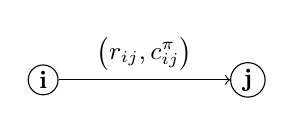
\begin{tikzpicture}[nodes={font=\bf\small}, scale=0.65]
%  \draw [help lines] (-1,-1) grid (8,5);o

\tikzstyle{tasknode}=[%
  draw,
  circle,
  minimum width=0.4,
  inner sep=0.5mm,
]

% nodes
\node [tasknode] (i) at (0, 0) {i};
\node [tasknode] (j) at (4, 0) {j};

\path [draw, ->] (i) -- node[above] {$\left(r_{ij},c_{ij}^{\pi}\right)$} (j);

\end{tikzpicture} 
%%%%%%%%%%%%%%%%%%%%%%%%%%%%%%%%%%%%%%%%%%%

        \caption{Notation: each arc is labelled with residual capacity and reduced cost.} 
        \label{fig:cs-trace:key}
    \end{subfigure}
    \begin{subfigure}[c]{0.5\textwidth}
        %%%%%%%%%%%%%%%%%%%%%%%%%%%%%%%%%%%%%%%%%%%
\begin{tikzpicture}[nodes={font=\bf\small}, scale=0.65]
%  \draw [help lines] (-1,-1) grid (8,5);o

\tikzstyle{tasknode}=[%
  draw,
  circle,
  minimum width=0.4,
  inner sep=0.5mm,
]

% T_0,0
\node [tasknode, black!70!green] (t00) at (0,6.5) {T$_0^0$};
% T_0,1
\node [tasknode, black!70!green] (t01) at (0,4.5) {T$_1^0$};

% X
\node [draw, rectangle, brown] (x) at (5.0,3.5) {X};

% M_0 & M_1
\node [draw, rectangle, blue] (m0) at (10.0,6.5) {M$_0$};
\node [draw, rectangle, blue] (m1) at (10.0,4.5) {M$_1$};
\node [draw, rectangle, blue] (m2) at (10.0,2.5) {M$_2$};

% sink
\node [draw, regular polygon, regular polygon sides=6] (s) at (12, 3.5) {S};

% U_0
\node [draw, rectangle, red] (u0) at (5.0,7.0) {U$^0$};

% Tasks to X
\path [draw, ->] (t00) -- node[below, sloped] {1} (x);
\path [draw, ->] (t01) -- node[below, sloped] {1} (x);

% Tasks to U_i
\path [draw, ->] (t00) -- node[above, sloped] {5} (u0);
\path [draw, ->] (t01) -- node[above, sloped] {5} (u0);

% X to machines
\path [draw, ->] (x) -- node[below, sloped] {} (m0);
\path [draw, ->] (x) -- node[below, sloped] {} (m1);
\path [draw, ->] (x) -- node[below, sloped] {} (m2);

% Machines to sink
\path [draw, ->, red] (m0) -- node[above, sloped] {} (s);
\path [draw, ->, red] (m1) -- node[below, sloped] {} (s);
\path [draw, ->] (m2) -- node[below, sloped] {} (s);

% U_i to sink
\begin{scope}[decoration={post length=4pt},rounded corners=4mm]
  \path [draw, ->] (u0) -- ++(1.5,0.5) -- node[below, sloped] {} ++(6,0) -- ++(1,-0.5) -- (s);
\end{scope}

% running tasks
\path [draw, ->, dotted, red] (t00) edge[out=-30, in=180, looseness=1] node[above, sloped] {1} (m0);
\path [draw, ->, dotted, red] (t01) edge[out=15, in=180, looseness=1] node[above, sloped] {1} (m1);

\end{tikzpicture} 
%%%%%%%%%%%%%%%%%%%%%%%%%%%%%%%%%%%%%%%%%%%

        \caption{Initial network. $Q = \left[A\right]$.}
        \label{fig:cs-trace:initial}        
    \end{subfigure}
    \begin{subfigure}[c]{0.5\textwidth}
        \input{figures/flow/cs/first}
        \caption{$\textproc{Discharge}(A)$: immediately calls $\textproc{Relabel}(A)$ as there are no outgoing arcs with negative reduced cost. $Q$ remains $\left[A\right]$, as $A$ is popped and then immediately pushed again.}
        \label{fig:cs-trace:first}
    \end{subfigure}
    \begin{subfigure}[c]{0.5\textwidth}
        %%%%%%%%%%%%%%%%%%%%%%%%%%%%%%%%%%%%%%%%%%%
\begin{tikzpicture}[nodes={font=\bf\small}, scale=0.45]
%  \draw [help lines] (-1,-1) grid (8,5);o

% epsilon=10
% Q=[A]  
% discharge A
% Push(A,B)  
% Q=[B]
% Push(A,C)
% Q=[B,C]

\tikzstyle{mynode}=[%
  draw,
  circle,
  minimum width=0.4,
  inner sep=0.5mm,
]

\tikzstyle{myarc}=[%
  draw,
  arrows={-Triangle[scale=1]},
  line width=1pt,
]

% nodes
\node [mynode] (a) at (0, 4) {A};
\node [mynode] (b) at (4, 8) {B};
\node [mynode] (c) at (4, 0) {C};
\node [mynode] (d) at (8, 4) {D};

% excesses
\node [left=0.75cm] at (0,4.3) {$e_A = 0$}; % A
\node [above=0.6cm] at (4,8) {$e_B = 2$}; % B
\node [below=0.2cm] at (4,0) {$e_C = 1$}; % C
\node [right=0.5cm] at (8,4.3) {$e_D = -3$}; % D

% potentials
\node [left=0.5cm] at (0,3.7) {$\pi_A = 11$}; % A
\node [above=0.15cm] at (4,8) {$\pi_B = 0$}; % B
\node [below=0.65cm] at (4,0) {$\pi_C = 0$}; % C
\node [right=0.5cm] at (8,3.7) {$\pi_D = 0$}; % D

\path [myarc] (b) -- node[above, sloped] {$(2,10)$} (a);
\path [myarc] (a) -- node[below, sloped] {$(2,-6)$} (c);
\path [myarc] (c) edge[bend right=20, looseness=1] node[above, sloped] {$(1,6)$} (a);
\path [myarc] (b) -- node[right] {$(5,1)$} (c);
\path [myarc] (b) -- node[above, sloped] {$(1,10)$} (d);
\path [myarc] (c) -- node[below, sloped] {$(5,1)$} (d);

\end{tikzpicture} 
%%%%%%%%%%%%%%%%%%%%%%%%%%%%%%%%%%%%%%%%%%%

        \caption{$\textproc{Discharge}(A)$: calls $\textproc{Push}(A,B)$ and $\textproc{Push}(A,C)$, leaving $Q = \left[B,C\right]$.}
        \label{fig:cs-trace:second}        
    \end{subfigure}
    \begin{subfigure}[c]{0.5\textwidth}
        \input{figures/flow/cs/third}
        \caption{$\textproc{Discharge}(B)$: immediately calls $\textproc{Relabel}(B)$, leaving $Q = \left[C,B\right]$.}
        \label{fig:cs-trace:third}
    \end{subfigure}
    \begin{subfigure}[c]{0.5\textwidth}
       \input{figures/flow/cs/fourth}
        \caption{$\textproc{Discharge}(C)$: immediately calls $\textproc{Relabel}(C)$, leaving $Q = \left[B,C\right]$.}
        \label{fig:cs-trace:fourth}
    \end{subfigure}
    \caption[Cost scaling in action with FIFO vertex queue]{Partial trace of FIFO \textproc{Refine} from \cref{algo:cost-scaling-first-active-refine}, depicting the residual network after each call to \textproc{Discharge}. Each node $i$ is labelled with its excess $e_i$ and potential $\pi_i$. $\epsilon$ is taken to be $10$, as would be the case on the first call to \textproc{Refine} from \cref{algo:cost-scaling} (note the maximum cost $C$ in the network is 10.)}
    \label{fig:cs-trace}
\end{figure}

\begin{algorithm}
\begin{algorithmic}[1]
    \Function{Refine}{$\mathbf{x}$,$\boldsymbol{\pi}$,$\epsilon$}
        \State initialisation as in lines 2-4 of \cref{algo:cost-scaling-generic-refine}
        \Let{$Q$}{$\left[s \in V \::\: e_s > 0\right]$} \Comment{$Q$ is a queue of excess vertices}
        \While{$Q$ not empty}
            \State pop head of $Q$ into $s$
            \State \Call{Discharge}{$s$,$\epsilon$} \Comment{May add vertices to $Q$}
            \If{\textproc{Relabel} called by \textproc{Discharge}}
                \State add $s$ to rear of $Q$
                \Break
            \EndIf
        \EndWhile
    \EndFunction
\end{algorithmic}
\caption{Cost scaling: FIFO \textproc{Refine} routine}
\label{algo:cost-scaling-first-active-refine}
\end{algorithm}

\Cref{algo:cost-scaling-first-active-refine} maintains a first-in-first-out (FIFO) queue $Q$ of excess vertices (see \cref{sec:prep-flow-pseudo}). The initial order of vertices in the queue is arbitrary. At each iteration, an excess vertex $s$ is removed from the head of the queue, and \emph{discharged} by applying a sequence of \textproc{Push} and \textproc{Relabel} operations (described below). During execution of the algorithm, new vertices may gain an excess; in this case, they are added to the rear of $Q$.

\begin{algorithm}
\begin{algorithmic}[1]
    \Require{$e_s > 0$}
    \Function{Discharge}{$s$,$\epsilon$}
        \Repeat
            \State \Call{PushOrRelabel}{$s$,$\epsilon$}
        \Until $e_s \leq 0$
    \EndFunction
    \stepcounter{algorithmicH}
    \setcounter{ALG@line}{0}
    \Statex
    \Require{$e_s > 0$}
    \Function{PushOrRelabel}{$s$,$\epsilon$}
        \State let $(i,j)$ be the current arc of $s$
        \If{$(i,j) \in E_\mathbf{x}$ and $c_{ij}^{\boldsymbol{\pi}} < 0$} \Call{Push}{$i$,$j$}
        \Else
            \If{$(i,j)$ last arc on the adjacency list for $s$}
                \State \Call{Relabel}{$s$}
                \Let{current arc}{first arc in adjacency list}
            \Else
                \Let{current arc}{next arc in adjacency list}
            \EndIf
        \EndIf
    \EndFunction
\end{algorithmic}
\caption{Cost scaling: \textproc{Discharge} and helper routine \textproc{PushOrRelabel}}
\label{algo:cost-scaling-discharge}
\end{algorithm}

$\textproc{Discharge}(s)$ is described in \cref{algo:cost-scaling-discharge}. It may be applied to any excess vertex, and performs a sequence of push operations until $e_s = 0$ or \textproc{Relabel} is called. For each vertex $i \in V$, an adjacency list is maintained, in a fixed (but arbitrary) order. The helper routine \textproc{PushOrRelabel} walks over this adjacency list, performing \textproc{Push} operations when possible. When the end of this adjacency list is reached, no further \textproc{Push} operations can be performed, and \textproc{Relabel} is invoked.

Note any new excess vertices generated during execution of the algorithm must be added to the rear of $Q$. $\textproc{Push}(i,j)$ may make $j$ an excess vertex: \cref{algo:cost-scaling-operations} must be modified to check for this case. The code for \textproc{Refine} in \cref{algo:cost-scaling-generic-refine} must also be updated. \textproc{Refine} pops $s$ from $Q$ and then calls \textproc{Discharge}. If \textproc{Relabel} is called by \textproc{Discharge}, $s$ will still be an active vertex when \textproc{Discharge} returns, and must be added back to the queue $Q$.

\Cref{fig:cs-trace} illustrates the operation of FIFO \textproc{Refine}, showing how each call to \textproc{Discharge} modifies the potentials $\mathbf{\pi}$ and flow $\mathbf{x}$ on a simple network.

\begin{thm} \label{thm:cost-scaling-first-active-complexity}
The algorithm with FIFO refine has a running time of $O(n^2m \lg (nC))$.
\end{thm}
\begin{proof}
See Goldberg and Tarjan~\cite[theorem~6.2]{Goldberg:1990}.
\end{proof}

\begin{remark}
In fact, this complexity bound holds for any refine routine which repeatedly applies \textproc{PushOrRelabel}. However, it has been conjectured by Goldberg that the FIFO ordering of vertices in this variant results in a tighter bound of $O(n^3 \lg (nC))$. Proving or disproving this assertion is an open research problem.\\
\end{remark} 

\begin{remark}
On flow scheduling networks, $m = O(n)$ by \cref{lemma:network-num-arcs}, so the bound is trivially $O(n^3 \lg (nC))$ in any case.
\end{remark}

\subsubsection{Wave refine} \label{sec:impl-cs-impl-wave}

\begin{algorithm}
\begin{algorithmic}[1]
    \Function{Refine}{$\mathbf{x}$,$\boldsymbol{\pi}$,$\epsilon$}
    \State initialisation as in lines 2-4 of \label{algo:cost-scaling-wave-refine:initialisation} \cref{algo:cost-scaling-generic-refine}
    \Let{$L$}{list of vertices in $V$} \Comment{order of vertices is arbitrary}
    \Repeat
        \For{each vertex $i$ in list $L$}
            \If{$e_i > 0$}
                \State \Call{Discharge}{$i$,$\epsilon$}
                \If{\textproc{Relabel} called by \textproc{Discharge}}
                    \State move $i$ to front of $L$
                \EndIf
            \EndIf
        \EndFor
    \Until{no excess vertex encountered in \textbf{for} loop}
    \EndFunction
\end{algorithmic}
\caption{Cost scaling: wave \textproc{Refine} routine}
\label{algo:cost-scaling-wave-refine}
\end{algorithm}

\Cref{algo:cost-scaling-wave-refine} describes an approach which can be proved to achieve the $O(n^3 \lg (nC))$ bound on any flow network. The method maintains a list $L$ of all vertices in the network, rather than the queue $Q$ maintained by the FIFO method. The algorithm preserves the invariant that $L$ is topologically ordered with respect to the \emph{admissible graph}: the subgraph of the residual network containing only arcs with negative reduced cost.

Initially, $L$ contains vertices in arbitrary order. But the admissible graph is empty after \cref{algo:cost-scaling-wave-refine:initialisation} of \cref{algo:cost-scaling-wave-refine}, since \crefrange{algo:cost-scaling-generic-refine:start-init}{algo:cost-scaling-generic-refine:end-init} of \cref{algo:cost-scaling-generic-refine} saturate any negative reduced cost arcs, making them drop out of the residual network. Thus, $L$ is trivially topologically ordered.

\textproc{Push} operations cannot create admissible arcs, and so preserve the topological ordering. An operation $\textproc{Relabel}(s)$ can create admissible arcs. However, there are guaranteed to be no admissible arcs entering $s$ immediately after the operation~\cite[lemma~6.5]{Goldberg:1987}. Moving $s$ to the beginning of $L$ therefore ensures a topological ordering is maintained.\\

\begin{thm} \label{thm:cost-scaling-wave-complexity}
The algorithm with wave refine has a running time of $O(n^3 \lg (nC))$.
\end{thm}
\begin{proof}
Using the invariant that $L$ is topologically ordered, it is possible to prove an $O(n^2)$ bound on the number of passes over the vertex list~\cite[lemma~7.3]{Goldberg:1987}. An $O(n^3)$ bound on the running time of the wave \textproc{Refine} routine can be shown as a corollary of this~\cite[theorem~7.4]{Goldberg:1987}. The result follows by \cref{lemma:cost-scaling-overall-algorithm}.
\end{proof}

\subsection{Heuristics}

So far, this dissertation has only considered means to improve the theoretical performance of cost scaling. Considerable research effort has gone into improving its practical performance by means of \emph{heuristics} that guide the actions of the algorithm~\cite{Goldberg:1997}.

I decided not to implement any heuristics. The heuristics are already well-studied: implementing them would not have produced any new insight, and would have diverted considerable development time from other efforts. I judged that it was better to keep my implementation simple, allowing me to rapidly explore fundamentally different approaches. However, for the sake of completeness I have summarised the heuristics in \cref{appendix:impl-csheuristics}.

% Optimisations: changing scaling factor, maintaining integrality, wave vs sequential
% Optimisations may be better left for evaluation? If you do want to include it here, should merge it into heuristics with a section e.g. Improving performance

\section{Approximation algorithms} \label{sec:impl-approx}

% PROOFREAD - Intro: 1 major edits, 2 minor edits

Feasible solutions to flow scheduling networks correspond to scheduling assignments. A solution's cost indicates the degree to which the assignment meets the scheduler's policy goals. The algorithms considered so far find \emph{minimal} cost flows, producing scheduling assignments which \emph{maximise} the policy objectives.

Finding the best solution may take some time, yet minimising scheduling latency is itself important (see \cref{sec:prep-scheduling}). I develop an approximate solution method, allowing the trade-off between accuracy and speed to be chosen explicitly.

% It may be possible to find an \emph{approximate} solution -- a flow with low, albeit not minimal, cost -- faster than an optimal solution. Whole-system performance may improve due to the reduction in scheduling latency, in spite of a less-than-optimal allocation of tasks.
%However, finding the best solution may take some time, yet minimising scheduling latency is itself an important objective (see \cref{sec:prep-scheduling}). It is wasteful for machines to run idle, waiting for tasks to be scheduled; moreover, interactive applications cannot tolerate high scheduling delays. I develop an \emph{approximate} solver, allowing the trade-off between scheduling accuracy and speed to be chosen explicitly.

I believe this is the first study of approximation algorithms for the minimum-cost flow problem. There is some prior work on finding approximate solutions for the related NP-complete problems of multi-commodity flows~\cite{Garg:2007} and dynamic flows~\cite{Hoppe:1994}. These techniques are of limited applicability to minimum-cost flow problems\footnotemark, however, and Hapi uses entirely different methods for approximation.
\footnotetext{For example, approximation methods for multi-commodity flow problems often work by solving many single-commodity flow problems. Obviously this reduction method does not help when the problem is already single-commodity.}

\subsection{Choice of algorithms} \label{sec:impl-approx-choice}

% PROOFREAD - 1 minor edits.
The solution returned by an approximate algorithm must be \emph{feasible}, although it need not be \emph{optimal}. Of the algorithms considered in sections \ref{sec:impl-cycle-cancelling} to \ref{sec:impl-cost-scaling}, only cycle cancelling and cost scaling maintain feasibility as an invariant\footnotemark.
\footnotetext{Successive shortest path and relaxation, by contrast, operate on a pseudoflow and maintain optimality as an invariant.}

Both cycle cancelling and cost scaling find successive approximations to an optimal solution, and so can readily be adapted to find approximate solutions. In cycle cancelling, the cost of the solution monotonically decreases after each iteration (shown in the proof of \cref{lemma:cycle-cancelling-termination}). However, a large decrease in the cost of the solution may occur at \emph{any} point in the algorithm's execution.

By contrast, in cost scaling the error bound $\epsilon$ undergoes exponential decay\footnotemark, reaching a small value many iterations before the algorithm would normally terminate. It will therefore produce a better approximation than cycle cancelling. Cost scaling is also considerably faster than cycle cancelling, making it the clear choice for an approximate solver.
\footnotetext{The solution cost \emph{tends} to also undergo exponential decay. However, this is not guaranteed: the error bound is not tight, and the cost on occasion may even increase.}

\subsection{Adapting cost scaling} \label{sec:impl-approx-adaptions}

% PROOFREAD - 1 major edits.
Cost scaling finds successive $\epsilon$-optimal solutions, where $\epsilon$ is decreased by a constant factor $\alpha$ after every iteration (see \cref{algo:cost-scaling}). It terminates when $\epsilon < 1/n$, at which point the solution is optimal by \cref{thm:epsilon-optimality-optimal}. Relaxing this terminating condition produces an approximate solver.

Ideally, it would be possible to specify a bound on the relative error of the solution: for example, terminating once the error is smaller than 1\%. Unfortunately, computing the relative error requires knowing the minimum cost, which can only be determined by finding an optimal solution.

It is possible to derive a bound on the absolute error of the solution, in terms of $\epsilon$. Unfortunately, the bound is of limited practical use. \Cref{defn:epsilon-optimality} of $\epsilon$-optimality has the simple corollary that:

\[\epsilon = \max_{(i,j) \in E_\mathbf{x}} -c_{ij}^{\boldsymbol{\pi}}\]

$\epsilon$ therefore depends on the `worst' arc in the residual network: i.e.\ the one with the most negative reduced cost. If every arc were to attain this worst case, the error could be large even for small values of $\epsilon$. But in practice, this does not occur. The bound therefore tends to significantly overestimate the solution error.

As accurate analytic bounds on the error are not available, I had to develop heuristic terminating conditions. These are the focus of the rest of this section.

% N.B. Commented out as never evaluated, and it's kind of a stupid heuristic anyway.
%\subsubsection{$\epsilon$ threshold}
%
%In this heuristic, the algorithm terminates as soon as $\epsilon$ drops below some fixed threshold. Note that setting the threshold to $1/n$ recovers the original algorithm.
%
%More sophisticated heuristics are expected to outperform this technique. However, as the simplest possible approach, it serves as a natural baseline for evaluation.

\subsubsection{Cost convergence}

\begin{figure}
    \centering
    \includegraphics{app/quincy_medium_over_time_2col}
    \caption[Successive approximations to an optimal solution.]{Successive approximations to an optimal solution. Each iteration of cost scaling is marked by a point on the graph. The spacing between points on the $x$-axis indicate the time taken by \textproc{Refine}. This varies throughout execution of the algorithm, but does not show any trend: \textproc{Refine} runs for a similar length of time immediately before optimality as for the first iteration. Note that the $y$-axis, representing solution cost, is on a log scale. The results are for a scheduling flow network from the dataset described in \cref{sec:eval-approx-flow-scheduling}.}
    \label{fig:app-cost-over-time}
\end{figure}

The first few iterations of cost scaling tend to produce large reductions in the cost. When the solution is nearly optimal, the change in cost between successive iterations is typically small. This is illustrated in \cref{fig:app-cost-over-time}, which shows cost scaling running on a scheduling flow network. 

Cost convergence exploits this property, by measuring the difference between the cost after successive iterations. If the cost changes by a factor less than some threshold $t$, the algorithm terminates.

%On some flow networks, cost scaling hits a brief `plateau', before continuing to make significant cost reductions. My implementation can optionally consider multiple prior iterations, terminating only when the cost change is below the threshold in the last $k \geq 1$ iterations, to combat this.

\subsubsection{Task migration convergence}

Cost convergence is a general approach, applicable to any class of flow network. By contrast, this heuristic exploits the nature of flow scheduling. Vertices are labelled as representing either a task, machine or other entity. Task assignments are computed from the flow (see \cref{sec:prep-flow-scheduling}), and the number of changes from the last iteration is measured. The algorithm terminates when this drops below a threshold $t$.

% Extensions: hybrid schemes? Error bounds based on arcs being fixed?

\section{Incremental algorithms} \label{sec:impl-incremental}

% PROOFREAD: 1 minor edits, 2 minor edits

% FIGURE: Sequence of flow graphs, showing small change?
Flow scheduling systems produce a sequence of closely related flow networks. Each new network in the sequence is generated in response to cluster events, such as task submission or completion. Most changes are highly localised in the flow network: consequently, the optimal flow remains mostly the same.

My method of \emph{incremental} solution is designed to exploit this. The algorithm reuses the solution for the old flow network, \emph{reoptimising} to produce an answer for the new network. This approach proved to be extremely successful, producing a factor of $14.5\times$ speedup in my tests (see \cref{sec:eval-incremental}). I believe my implementation is the first of its kind: there is certainly no mention of this method in the literature.

Flow scheduling is ideally suited to an incremental solution method. However, the approach is much less compelling for traditional applications of flow networks: this may go some way to explaining the lack of prior work. As previously mentioned, most network changes in flow scheduling are small. This alone does not make the problem easy: reoptimising after even a single change is, in general, as hard as solving the problem from scratch\footnotemark. Informally, the problem is that since the optimisation problem is global, an update in one region of the network may trigger a cascading sequence of changes in the optimal flow for distant regions.
\footnotetext{To see this, consider two networks $A$ and $B$. WLOG, assume they each have a single supply vertex $s_x$ and demand vertex $t_x$ for $x \in {A,B}$. Remove the supply and demand at those vertices, introducing new supply and demand vertices $s$ and $t$. Add arcs $s\to s_x$ with capacity $b_{s_x}$, and $t_x \to t$ with capacity $-b_{t_x}$, for $x \in {A,B}$. Let $C$ be a cost larger than the cost of any flow in networks $A$ or $B$; set the cost of $s \to s_A$ to $C$ and $s \to s_B$ to $2C$. The resulting network is effectively equivalent to just network $A$. Dropping the cost on $s \to S_B$ from $2C$ to $0$ makes the resulting network effectively equivalent to $B$. Solving this incremental change is thus as hard as solving the entire network $B$.}

Crucially, however, scheduling policies are designed to produce stable assignments of tasks to machines. Preempting a task is an expensive operation, which should be performed sparingly. Consequently, the cost model for any viable scheduling policy naturally avoids frequent changes to the optimal flow. This is precisely the property required for incremental solvers to perform well.

I describe the sources I drew on to develop my incremental solver in the next section, \cref{sec:impl-incremental-related-work}. Following this, I discuss my approach to building such a solver in \cref{sec:impl-incremental-architecture}. After this background, I evaluate the suitability of different flow algorithms to the incremental problem in \cref{sec:impl-incremental-choice}. Following this, \cref{sec:impl-incremental-impl} provides details of the solvers I implemented.

\subsection{Related work} \label{sec:impl-incremental-related-work}
The Quincy paper highlighted incremental solvers as an area for further research, sparking my interest in such an approach~\cite[\S6.5]{Isard:2007}. There has been some study of reoptimisation and sensitivity analysis on flow networks, which are related to the incremental problem, although these areas have received comparatively little attention. I survey the existing work below.

Amini and Barr published a comprehensive empirical evaluation of reoptimisation algorithms in 1993~\cite{Amini:1993}. However, the study tested algorithms such as the out-of-kilter method, now long obsolete. Moreover, the largest network studied had only 1,500 vertices, orders of magnitude smaller than the ones considered in this project. 

The most recent work is a computational study of algorithms for reoptimisation after arc cost changes, published by Frangioni and Manca in 2006~\cite{Frangioni:2006}. Although now almost a decade old, the algorithms evaluated are still in contemporary use. However, the results of the study may not generalise to flow scheduling, where any parameter -- not just arc costs -- can change. 

Sensitivity analysis on flow networks seeks to determine how uncertainty in network parameters causes uncertainty in the optimal solution~\cite[\S9.11]{Ahuja:1993}. In scientific applications, this may be used to test the robustness of a flow model. Small changes in the input should produce similarly small changes in the output: otherwise, the model is too sensitive to measurement error. Although the goals of sensitivity analysis are considerably different to those of an incremental solver, some of the underlying techniques can be adapted.

\subsection{Architecture of an incremental algorithm} \label{sec:impl-incremental-architecture}

Previous sections in this chapter described the implementation of pre-existing algorithms. These are designed to solve the minimum-cost flow problem ``from scratch'': finding an optimal solution without the benefit of any existing state. An obvious incremental approach is to simply rerun one of these algorithms on the updated network, using the previous state as a starting point.

This does not quite work, however: most flow algorithms maintain an invariant on the state of the solver during intermediate computations. After a network update, this invariant may fail to hold. When the invariant is a precondition for the algorithm, as in relaxation, reoptimisation might fail entirely. In other algorithms, such as cost scaling, the invariant is used only to prove complexity bounds. Reoptimisation will succeed, but may run slower than expected.

Consequently, I adopt a three-step approach for my incremental algorithm:

\begin{enumerate}
    \item Receive changes to the flow network, updating any internal data structures.
    \item Manipulate the saved state, to satisfy the invariant under the updated network.
    \item Run the algorithm to reoptimise.
\end{enumerate}

In practice, implementation of this approach is considerably more challenging than suggested by this summary. Step 1 superficially appears trivial, but many graph data structures cannot be efficiently modified. Considerable research effort has gone into devising \emph{dynamic} data structures to resolve this problem~\cite{Tarjan:1983,Eppstein:1996}. In addition to the network itself, many algorithms rely on auxiliary data structures\footnotemark, which must also be updated.
\footnotetext{For example, many algorithms maintain a set of excess vertices to improve performance.}

Step 2 varies considerably between algorithms, and is discussed in \cref{sec:impl-incremental-impl}. Somewhat ironically, step 3 is the simplest, with the core of the algorithm remaining mostly unmodified. Since step 2 ensures that the invariant holds, the optimisation procedure can be run as usual after disabling any initialisation code.

\subsection{Choice of algorithms} \label{sec:impl-incremental-choice}
The approach suggested above could be applied to any flow algorithm considered in this dissertation. In this section, I consider which algorithms are most suited to operating incrementally. I start with cost scaling, which has excellent performance on the from scratch problem (see \cref{sec:impl-cost-scaling}). Next, I consider successive shortest path and relaxation (see \cref{sec:impl-ssp} and \cref{sec:impl-relax}). I do not discuss cycle cancelling, as it is considerably slower than the other algorithms.

\subsubsection{Cost scaling} 
%WORDCOUNT: Incremental choice of algorithm -- could make cuts to cost scaling
Despite excellent performance on the full problem, Goldberg's cost scaling algorithm fares poorly on the incremental problem. 

Cost scaling maintains the invariant that $\mathbf{x}$ is a feasible flow and $\left(\mathbf{x},\boldsymbol{\pi}\right)$ is $\epsilon$-optimal. This invariant is not required for correctness, but is needed for proofs of its complexity.

The starting state may be neither feasible nor optimal on the new network. To satisfy the invariant, feasibility must first be restored, such as by running a max-flow algorithm\footnotemark, which will tend to make the flow less optimal.
\footnotetext{In fact, it is perfectly legitimate to skip this stage and run \textproc{Refine} directly, which will also restore feasibility. However, the analysis is clearer when considering these stages separately.}

Next, the value of $\epsilon$ for which $\left(\mathbf{x},\boldsymbol{\pi}\right)$ is $\epsilon$-optimal must be calculated. This can be computed by a single pass over the arcs in the residual network. Alternatively, the potential refinement heuristic described in \cref{appendix:impl-csheuristics-potential-refinement} could be used: this might find a smaller value of $\epsilon$ by updating the potentials $\boldsymbol{\pi}$.

% I'm not sure that restoring feasibility does break $\epsilon$-optimality. We can just invoke Refine on the non-feasible flow, that's fine I think.
The key problem is that $\epsilon$ may be very large even after a small update. Recall that $\epsilon$-optimality (see \cref{defn:epsilon-optimality}) is defined as a property satisfied by \emph{every} arc. $\epsilon$ is thus a measure of the \emph{maximum} error in the solution. An update as simple as changing the cost on a single arc can make $\epsilon$ large, even though the rest of the network remains $0$-optimal. Since $\epsilon$ often ends up close (in logarithmic terms) to its starting value $C$, the algorithm performs almost as many iterations of \textproc{Refine} as it would in the full case.
% Below is good, but wordcount.
% Furthermore, there is no reason to hope the iterations will complete any faster than usual. Although \textproc{Refine} maintains $\epsilon$-optimality, it can make previously optimised segments of the network \emph{less} optimal (up to the bound of $\epsilon$), effectively creating more work for future iterations.

%WONTFIX: Would be interesting to try and model the performance of CS2. Simple approach which could work: assume new epsilon is ~U[0,C], what is the mean and variance of log_2 (C/epsilon)?
The computational study of cost reoptimisation by Frangioni and Manca~\cite{Frangioni:2006} supports my assertion. Whereas other algorithms enjoyed speedups of $20\times$ or more, cost scaling had only a $2\times$ speedup. Moreover, its performance was unpredictable, varying considerably even within networks of the same class.

\subsubsection{Successive shortest path and relaxation}

Both the successive shortest path and relaxation algorithm work by sending flow along \emph{augmenting paths}. These paths start at an excess vertex, and reach an excess vertex traversing only arcs of zero or negative reduced cost. Although the two algorithms differ considerably, they have similar incremental properties. In particular, note they both maintain the invariant that $\left(\mathbf{x},\boldsymbol{\pi}\right)$ satisfies reduced-cost optimality conditions, seeking to successively improve the feasibility of $\mathbf{x}$\footnotemark.
\footnotetext{This is most clear in the successive shortest path algorithm, which improves the feasibility of $\mathbf{x}$ on every iteration. It is not strictly speaking the case for the relaxation algorithm, since the the \textproc{UpdatePotentials} operation may make the flow \emph{less} feasible. But, indirectly, \textproc{UpdatePotentials} is still working towards feasibility since it allows for more \textproc{AugmentFlow} operations to take place.}

Changes to the network can violate reduced cost optimality, but the pseudoflow can be modified inexpensively to maintain optimality (see \cref{sec:impl-incremental-maintaining-rc} for my method). The algorithm can then be run as usual to reoptimise, restoring feasibility. This takes time proportional to the reduction in feasibility of the solution caused by the updates\footnotemark. This is a very desirable property for flow scheduling, where most changes will only impact the feasibility of a small region of the network.
\footnotetext{Note that the feasibility may be reduced directly and indirectly. Direct decreases in feasibility occur as an immediate consequence of a network update: for example, adding a new source and sink vertex. The feasibility may also be compromised indirectly: the operations needed to maintain reduced cost optimality might require pushing flows along arcs, resulting in excesses or deficits at vertices.}

The relaxation algorithm is evaluated empirically in the study by Frangioni and Manca. As I discussed in \cref{sec:impl-relax}, the practical performance characteristics of the algorithm are heavily dependent on the class of problem. This is apparent from the study: relaxation is competitive on the NETGEN, GRIDGEN and GOTO instances but performs poorly on PDS instances~\cite[tables~1~to~4]{Frangioni:2006}. Relaxation is fast on flow scheduling networks even as a from scratch solver (see \cref{fig:inc-same:relax-my}), so there are reasons to be optimistic about its incremental performance. 

There are no benchmarks in the literature for reoptimisation using successive shortest path. However, since it belongs to the same class of algorithms as relaxation, I would predict a similar relative speedup. 

To conclude, there are substantial theoretical and practical reasons to favour the augmenting path algorithms. Based on this support, I decided to implement incremental versions of successive shortest path and relaxation, described further in \cref{sec:impl-incremental-impl}.

\subsection{Maintaining reduced cost optimality} \label{sec:impl-incremental-maintaining-rc}

Augmenting path algorithms maintain the invariant that $\left(\mathbf{x},\boldsymbol{\pi}\right)$ satisfies reduced cost optimality conditions, that is:
\[\forall(i,j)\in E_{\mathbf{x}}\cdot c_{ij}^{\boldsymbol{\pi}}\geq 0.\]
In from scratch optimisation, both $\mathbf{x}$ and $\boldsymbol{\pi}$ are initialised to $\mathbf{0}$, guaranteeing these conditions hold. When reoptimising, it is the responsibility of the caller to ensure the starting state satisfies the invariant.

In this section, I describe the method I developed to restore reduced cost optimality after the network is updated. Note the pseudoflow $\mathbf{x}$ may become less feasible as a side-effect of this procedure, although I minimise this where possible. The routine only modifies the pseudoflow $\mathbf{x}$: the potential $\pi_i$ of an existing vertex $i \in V$ is never changed.

\subsubsection{Vertex updates}

Adding or removing a vertex without arcs cannot violate reduced cost optimality, as $E_\mathbf{x}$ is unchanged. Of course, a vertex is added or removed along with its associated arcs, but arc updates are considered in the next section. It follows that no action need be taken on vertex removal. When a vertex $i$ is added, the potential vector $\boldsymbol{\pi}$ must be extended to include an element $\pi_i$. The choice of the value $\pi_i$ is arbitrary: it is initialised to zero in my implementation.

It is also possible to change the supply or demand $b_i$ of an existing vertex $i \in V$. Since this does not change the reduced cost of any arc, it cannot violate the optimality conditions, so no action is taken.

\subsubsection{Adding or removing an arc}

Note that having an arc $(i,j) \in E$ of zero capacity is equivalent to having no such arc in the network, $(i,j) \not \in E$. In both cases, the flow $x_{ij}$ is always zero, and the arc is absent from the residual network: $(i,j) \not \in E_\mathbf{x} \land (j,i) \not \in E_\mathbf{x}$.

Adding or removing an arc thus reduces to changing the capacity on the arc, covered in the next section. Removing an arc $(i,j)$ is equivalent to decreasing its capacity to $0$. The addition of an arc $(i,j)$ with cost $c_{ij}$ and capacity $u_{ij}$ can be modelled as updating increasing the capacity of an arc $(i,j)$ with cost $c_{ij}$ from $0$ to $u_{ij}$.

\subsubsection{Updating arc capacity}

Changing the capacity of an arc $(i,j)$ from $u_{ij}$ to $u'_{ij}$ does not change $c_{ij}$ or the potentials $\boldsymbol{\pi}$. The reduced cost $c_{ij}^{\boldsymbol{\pi}}$ therefore remains unchanged. However, it may be necessary to update $x_{ij}$. The procedure depends on whether the capacity is increasing, or decreasing.

\begin{itemize}
    \item \textbf{Decreasing capacity.} Set $x_{ij} \gets \min\left(x_{ij},u'_{ij}\right)$ to ensure the capacity constraints of \cref{eq:capacity-constraints} continue to hold\footnotemark. The below case analysis shows this preserves reduced cost optimality.
    \footnotetext{Whilst the primary goal of this method is to preserve reduced cost optimality, a more primitive requirement is that $\mathbf{x}$ continues to be a pseudoflow!}
    
    Suppose $(i,j) \not \in E_\mathbf{x}$: the arc was not present in the residual network prior to the update. Then the arc was previously saturated, with $x_{ij} = u_{ij}$, and $x_{ij} = u'_{ij}$ now holds. Thus the arc remains saturated, and so $(i,j) \not \in E_\mathbf{x}$ is still true.
    
    Otherwise, $(i,j) \in E_\mathbf{x}$. Since reduced cost optimality was satisfied prior to the update, $c_{ij}^{\boldsymbol{\pi}} \geq 0$ must have held. Since $c_{ij}^{\boldsymbol{\pi}}$ is not changed by the procedure, this will continue to hold. Note that if $x_{ij} \geq u'_{ij}$, then $(i,j) \not \in E_\mathbf{x}$ after the update, but this is harmless.
    \item \textbf{Increasing capacity.} There are two cases to consider. If $c_{ij}^{\boldsymbol{\pi}} \geq 0$, then no action need be taken. However, if $c_{ij}^{\boldsymbol{\pi}} < 0$ then $x_{ij}$ must be set to $u'_{ij}$, so that $(i,j)$ remains absent from the residual network.
\end{itemize}

\subsubsection{Updating arc cost}

Changing the cost of an arc $(i,j)$ from $c_{ij}$ to $c'_{ij} = c_{ij} + \delta$ changes the reduced cost from $c_{ij}^{\boldsymbol{\pi}}$ to $c_{ij}^{\prime\boldsymbol{\pi}} = c_{ij}^{\boldsymbol{\pi}} + \delta$. It is simplest to consider the complementary slackness conditions of \cref{eq:optimality-complementary-slackness}, which are equivalent to the reduced cost conditions of \cref{eq:optimality-reduced-cost} by \cref{thm:optimality-complementary-slackness}.

\begin{enumerate}
    \item \textbf{Case $c_{ij}^{\prime\boldsymbol{\pi}} > 0$:} set $x_{ij} \gets 0$. Note that this will already be the case if $c_{ij}^{\boldsymbol{\pi}} > 0$.
    \item \textbf{Case $c_{ij}^{\prime\boldsymbol{\pi}} = 0$: } this case is a no-op. Complementary slackness is satisfied for all values of $x_{ij}$ satisfying the capacity constraints $0 \leq x_{ij} \leq u_{ij}$.
    \item \textbf{Case $c_{ij}^{\prime\boldsymbol{\pi}} < 0$: } set $x_{ij} \gets u_{ij}$. Note that this will already be the case if $c_{ij}^{\boldsymbol{\pi}} < 0$.
\end{enumerate}

\subsection{Implementations} \label{sec:impl-incremental-impl}

I developed three incremental solvers. I adapted my implementations of the successive shortest path and relaxation algorithm, described in \cref{sec:impl-ssp} and \cref{sec:impl-relax}, to support incremental operation. In addition, I extended RELAX-IV~\cite{BertsekasCodes:1988,RelaxIV:2011} --- a highly optimised reference implementation of the relaxation algorithm --- to operate incrementally.

\subsubsection{Extending this project's implementations}
It proved relatively straightforward to modify my existing implementations of successive shortest path and the relaxation algorithm. This reflects the emphasis placed on modularity and design flexibility during earlier development.

The method to preserve reduced cost optimality, described in \cref{sec:impl-incremental-maintaining-rc}, was implemented using a wrapper class encapsulating graph objects. The wrapper first updates the flow to maintain optimality, and then forwards the changes to the underlying graph object.

Since the wrapper provides the same interface as the graph classes, it can be used as a drop-in replacement. This minimises the changes needed in the rest of the codebase. The algorithms themselves required little modification: I merely added a flag to disable the initialisation routine when operating incrementally.
 
\subsubsection{Extending RELAX-IV}
%WORDCOUNT: Extending RELAX-IV -- could probably make further cuts here
The RELAX-IV solver was considerably more challenging to modify. Whereas this project's implementations attempted to strike a balance between flexibility and efficiency, performance was the overriding objective for RELAX-IV. 

The source code is 5,000 lines in total, with some individual functions longer than 800 lines. The original Fortran version of the code is due to Bertsekas, and dates to 1988~\cite{BertsekasCodes:1988}. I worked with a C++ port by Frangioni and Gentile from 2003~\cite{RelaxIV:2011}.

%Although this port made integration with the rest of my project somewhat easier, many of the foibles of the original code remain, and some new ones were introduced.

Frangioni had already added support for cost reoptimisation for his aforementioned computational study~\cite{Frangioni:2006}. It appears he started to add support for other forms of updates; however, this development must have been interrupted, since my testing uncovered numerous bugs. The large, legacy codebase made these time consuming to fix. I intend to report the bugs discovered to the authors, making my patches available.

The rest of the changes I made were comparatively straightforward. RELAX-IV allocated data structure memory statically. This is problematic for an incremental solver, as the size of the network is not known in advance. I added support to dynamically resize the data structures, employing the usual strategy of exponential growth in size to achieve memory allocation in amortized linear time\footnotemark.
\footnotetext{Spikes in scheduling latency are undesirable, even if the average latency remains low. Since the solver is nowhere close to exhausting available memory, my implementation initially allocates twice as much memory as currently needed, in a bid to avoid needing to ever grow the array.}

RELAX-IV does not reuse vertex identifiers, causing a memory leak. I modified the algorithm to maintain a set of free vertices. New vertices are allocated an identifier from this set, with the underlying data structures expanded only when there are no free vertices.

Each arc $(i,j)$ is identified by an array index in RELAX-IV. Of course, the flow scheduling system is not privy to this internal index, and can only identify arcs by their source and destination vertices $i$ and $j$. Finding the index requires scanning the adjacency list of $i$ to find the arc to $j$ (or vice-versa), an $O(n)$ operation. My implementation makes a time-memory tradeoff, maintaining a hash table mapping pairs $(i,j)$ to indices, providing $O(1)$ lookups.

%\section{Input and output}
%
%% Drop this section if short of space, or punt to appendix. Optimisations probably the most useful/interesting ones to talk about.
%
%Loading networks, exporting results. Neither interesting nor impressive, but it is a necessary part of the project. Keep it brief. (Or cut it entirely?)
%
%\subsection{DIMACS}
%
%Representation for network, and network solution. Justify why: standard, widely used, readily available test data, integration with Firmament. 
%
%\subsection{Incremental extension}
%
%Why DIMACS isn't suitable for incremental problem: reloading the graph and computing diff prohibitive cost. 
%
%\subsection{Parser optimisations}
%
%Ignore zero-capacity arcs. Entirely trivial, but did produce noticeable performance improvement. Maybe worth mentioning.
%
%Ignoring duplicates. Necessary for correctness. Slightly more interesting: checking whether an arc is present is slow in some data structures (where the corresponding algorithm doesn't require manual lookup). Parser maintains a bitmap instead to check this quickly irrespective of data structure. Considerable performance improvement. 
%
%\subsection{Scheduling tasks}
%
%Show how solver can achieve original task, by integrating into a cluster scheduler. Choice of Firmament: can be briefly justified, but need not be at all (no real alternatives).

\section{Extensions to Firmament} \label{sec:impl-firmament}

% PROOFREAD: None

% FIGURE: scope of Firmament extension? XXX [good to get credit for this, & relatively easy]

The last two sections described my implementation of approximate and incremental solution methods. This section considers their use as part of a flow scheduling platform, Firmament~\cite[ch.~5]{Schwarzkopf:2015}. Integration with Firmament was straightforward: the standard DIMACS format is used to exchange flow networks and their solution~\cite{DIMACSStandard}. However, I significantly extended Firmament in other ways.

The most substantial change was adding support for incremental solvers. Although Firmament already generated incremental updates to the flow network, the vast majority of such updates were spurious\footnotemark. Parsing the changes took longer than reoptimising! I patched the Firmament to generate only authentic changes, considerably improving performance.
\footnotetext{For example, arc change events were generated for every arc from a task to an unscheduled aggregator, irrespective of whether any parameters had changed.}

I implemented other extensions to assist performance evaluation. Firmament includes a cluster \emph{simulator}, allowing experiments to be conducted on a virtual cluster. However, the simulator was never intended to evaluate flow schedulers, and required substantial modification.

The simulator only supported the Octopus cost model, a simplistic policy which merely balances the load across machines (see \cref{sec:eval-benchmark-strategy-octopus}). I implemented the Quincy cost model, described in \cref{sec:prep-flow-scheduling}, to provide a more realistic basis for comparison. This required building entirely new simulated components, such as a distributed filesystem, described further in \cref{sec:eval-benchmark-strategy-quincy}.

I made various other minor extensions: for example, building a statistics module to record scheduling latency and other properties of the cluster, such as the number of running tasks. Moreover, I added numerous configuration options to the simulator: for example, allowing the number of machines in the cluster to be varied.

% Not mentioned:
%  - New termination conditions: number of events, number of rounds
%  - Hash: configurable \% of events
%  - Bugfixes: Don't rerun when no changes take place
% But OK to be brief!

\section{Summary}

This chapter began by summarising several standard flow algorithms which were implemented in this project. Next, I turned my attention to how these algorithms may be extended to improve performance on the flow scheduling problem. In \cref{sec:impl-approx}, I described how I modified the cost scaling algorithm to build an approximate solver, allowing accuracy to be traded for speed. In \cref{sec:impl-incremental}, I modified the successive shortest path and relaxation algorithm to operate incrementally. As far as I am aware, both implementations are the first of their kind.

I concluded with a summary of the extensions I made to the Firmament flow scheduling system, including adding support for the Quincy cost model. In the next chapter, I demonstrate the considerable speedup that results from using the solvers developed in this project with Firmament.